\documentclass[12pt,a4paper]{article}

% Márgenes y formato de párrafo
\usepackage[left=2.5cm,right=2.5cm,top=2.5cm,bottom=2.5cm]{geometry}
\setlength{\parindent}{0in}
\setlength{\parskip}{0.5\baselineskip}

% Paquetes esenciales
\usepackage[spanish]{babel}
\usepackage[utf8]{inputenc}
\usepackage[T1]{fontenc}
\usepackage{amsmath,amssymb,amsfonts,amsthm}
\usepackage{graphicx}
\usepackage[colorlinks=true,linkcolor=blue,urlcolor=blue,citecolor=blue]{hyperref}
\usepackage{caption,subcaption}
\usepackage{multicol,multirow}
\usepackage{xcolor}
\usepackage{enumitem}
\usepackage{booktabs}
\usepackage{float}
\usepackage{tocloft}
\usepackage{fancyhdr}
\usepackage{pgfplots}
\usepackage{listings}
\pgfplotsset{compat=1.18}

% Configuración de páginas
\pagestyle{fancy}
\fancyhf{}
\fancyhead[L]{\small Algoritmos de Alineamiento de Secuencias}
\fancyhead[R]{\small CC0F3 - Práctica 02}
\fancyfoot[C]{\thepage}

% Configuración del índice
\renewcommand{\cftsecleader}{\cftdotfill{\cftdotsep}}
\renewcommand*\contentsname{Contenido}

% Configuración de listas
\setlist[itemize]{itemsep=0.3em, topsep=0.5em}
\setlist[enumerate]{itemsep=0.3em, topsep=0.5em}

% Definición de colores personalizados
\definecolor{fondecytblue}{RGB}{41,128,185}
\definecolor{fondecytgreen}{RGB}{39,174,96}
\definecolor{codebackground}{RGB}{245,245,245}

% Configuración de código
\lstset{
    backgroundcolor=\color{codebackground},
    basicstyle=\ttfamily\small,
    breaklines=true,
    captionpos=b,
    frame=single,
    numbers=left,
    numberstyle=\tiny\color{gray},
    keywordstyle=\color{blue},
    commentstyle=\color{green!60!black},
    stringstyle=\color{red}
}

% -------------------------
% DOCUMENTO
% -------------------------

\begin{document}
\selectlanguage{spanish}

% -------------------------
% PORTADA
% -------------------------
\begin{titlepage}
\centering
\vspace*{1cm}

{\huge\bfseries Biología Computacional\par}
\vspace{0.5cm}
{\LARGE Algoritmos de Alineamiento de Secuencias\par}
\vspace{0.3cm}
{\Large Needleman-Wunsch y Smith-Waterman\par}

\vspace{2cm}

{\Large\textbf{Autor:}\par}
\vspace{0.5cm}
{\large Guillermo Ronie Salcedo Alvarez\par}

\vspace{1cm}


\includegraphics[width=0.3\textwidth]{img/logo_uni.png}
\vspace{1cm}

{\large Universidad Nacional de Ingeniería\\
Facultad de Ciencias\par}

\vspace{1cm}

{\large Curso: CC0F3 - Biología Computacional\\
Práctica 02\par}

\vfill

{\large Octubre 2025\par}

\end{titlepage}

% -------------------------
% RESUMEN
% -------------------------
\newpage
\thispagestyle{empty}

\begin{abstract}
\noindent
Este documento presenta la documentación de diseño e implementación de dos algoritmos fundamentales en bioinformática para el alineamiento de secuencias biológicas: Needleman-Wunsch (alineamiento global) y Smith-Waterman (alineamiento local). Ambos algoritmos utilizan programación dinámica para encontrar el alineamiento óptimo entre dos secuencias, pero difieren en su enfoque y aplicaciones.

Se describe la arquitectura del software desarrollado en Python, incluyendo las estructuras de datos, el diseño de clases, la complejidad algorítmica y los casos de prueba implementados. La implementación incluye visualización de matrices de scoring, generación de alineamientos con formato legible y exportación de resultados. Se presentan resultados experimentales con secuencias biológicas reales (hemoglobina e insulina) que demuestran la efectividad de ambos algoritmos en diferentes escenarios.

\vspace{0.5cm}
\noindent\textbf{Palabras clave:} Alineamiento de secuencias, Needleman-Wunsch, Smith-Waterman, programación dinámica, bioinformática, Python

\end{abstract}


\newpage
\pagenumbering{roman}
\tableofcontents

\newpage
\pagenumbering{arabic}

% -------------------------
% INTRODUCCIÓN
% -------------------------
\section{Introducción}

El alineamiento de secuencias es una técnica fundamental en bioinformática que permite comparar secuencias de ADN, ARN o proteínas para identificar regiones de similitud que pueden indicar relaciones funcionales, estructurales o evolutivas. Esta técnica tiene aplicaciones en diversos campos como la genómica comparativa, la predicción de estructura de proteínas, el diseño de fármacos y el estudio de la evolución molecular.

Existen dos enfoques principales para el alineamiento de secuencias:

\begin{itemize}
    \item \textbf{Alineamiento Global}: Busca el mejor alineamiento entre dos secuencias completas de principio a fin. Es útil cuando las secuencias tienen longitudes similares y se espera que estén relacionadas en toda su extensión.
    
    \item \textbf{Alineamiento Local}: Identifica las regiones de mayor similitud entre dos secuencias, ignorando las regiones no relacionadas. Es más apropiado cuando las secuencias tienen longitudes muy diferentes o solo comparten dominios conservados.
\end{itemize}

Este documento presenta el diseño e implementación de los dos algoritmos clásicos de programación dinámica para alineamiento de secuencias:

\begin{enumerate}
    \item \textbf{Needleman-Wunsch (1970)}: Algoritmo para alineamiento global óptimo.
    \item \textbf{Smith-Waterman (1981)}: Algoritmo para alineamiento local óptimo.
\end{enumerate}

\subsection{Objetivos}

\textbf{Objetivo General:}

Diseñar, implementar y documentar los algoritmos de Needleman-Wunsch y Smith-Waterman en Python, incluyendo visualización de resultados y casos de prueba con secuencias biológicas reales.

\textbf{Objetivos Específicos:}

\begin{enumerate}
    \item Comprender los fundamentos teóricos de la programación dinámica aplicada al alineamiento de secuencias.
    \item Diseñar una arquitectura de software modular y extensible para implementar ambos algoritmos.
    \item Implementar el algoritmo de Needleman-Wunsch para alineamiento global.
    \item Implementar el algoritmo de Smith-Waterman para alineamiento local.
    \item Desarrollar funciones de visualización para matrices de scoring y alineamientos resultantes.
    \item Validar la implementación con casos de prueba utilizando secuencias biológicas reales.
    \item Comparar el comportamiento y resultados de ambos algoritmos en diferentes escenarios.
\end{enumerate}

\subsection{Alcance}

La implementación cubre:

\begin{itemize}
    \item Algoritmos de alineamiento por pares (pairwise alignment) de secuencias.
    \item Sistema de puntuación lineal (match, mismatch, gap).
    \item Visualización de matrices de scoring.
    \item Generación de alineamientos con notación estándar (matches, mismatches, gaps).
    \item Exportación de resultados a archivos de texto.
    \item Casos de prueba con proteínas (hemoglobina, insulina).
\end{itemize}

% -------------------------
% MARCO TEÓRICO
% -------------------------
\section{Marco Teórico}

\subsection{Programación Dinámica}

La programación dinámica es un paradigma de diseño de algoritmos que resuelve problemas complejos dividiéndolos en subproblemas más simples y almacenando los resultados de estos subproblemas para evitar recalcularlos. Los algoritmos de alineamiento de secuencias son ejemplos clásicos de aplicación de programación dinámica.

\textbf{Principios fundamentales:}

\begin{enumerate}
    \item \textbf{Subestructura óptima}: La solución óptima del problema contiene soluciones óptimas de subproblemas.
    \item \textbf{Solapamiento de subproblemas}: Los mismos subproblemas se resuelven múltiples veces.
    \item \textbf{Memoización}: Almacenar resultados de subproblemas en una tabla (matriz) para reutilizarlos.
\end{enumerate}

\subsection{Sistema de Puntuación}

El alineamiento de secuencias requiere un sistema de puntuación para evaluar la calidad del alineamiento:

\begin{equation}
\text{Score} = n_{\text{match}} \cdot s_{\text{match}} + n_{\text{mismatch}} \cdot s_{\text{mismatch}} + n_{\text{gap}} \cdot s_{\text{gap}}
\end{equation}

Donde:
\begin{itemize}
    \item $s_{\text{match}}$: Puntuación por coincidencia (típicamente +1)
    \item $s_{\text{mismatch}}$: Penalización por sustitución (típicamente -1)
    \item $s_{\text{gap}}$: Penalización por inserción/deleción (típicamente -2)
\end{itemize}

\subsection{Complejidad Computacional}

Ambos algoritmos tienen:

\begin{itemize}
    \item \textbf{Complejidad temporal}: $O(m \times n)$ donde $m$ y $n$ son las longitudes de las secuencias.
    \item \textbf{Complejidad espacial}: $O(m \times n)$ para almacenar la matriz de scoring.
\end{itemize}

Esto los hace factibles para secuencias de longitud moderada (hasta miles de caracteres) pero computacionalmente costosos para secuencias muy largas o búsquedas en bases de datos.

% -------------------------
% DISEÑO E IMPLEMENTACIÓN
% -------------------------
\section{Diseño de los Algoritmos}

\subsection{Needleman-Wunsch: Alineamiento Global}

\subsubsection{Descripción del Algoritmo}

El algoritmo de Needleman-Wunsch, publicado en 1970, fue el primer algoritmo de programación dinámica aplicado al alineamiento de secuencias biológicas. Garantiza encontrar el alineamiento global óptimo entre dos secuencias completas.

\subsubsection{Fases del Algoritmo}

\textbf{1. Inicialización de la Matriz}

Se crea una matriz $M$ de dimensiones $(m+1) \times (n+1)$ donde:

\begin{align}
M[0][0] &= 0 \\
M[i][0] &= i \cdot s_{\text{gap}} \quad \text{para } i = 1 \ldots m \\
M[0][j] &= j \cdot s_{\text{gap}} \quad \text{para } j = 1 \ldots n
\end{align}

\begin{figure}[H]
\centering
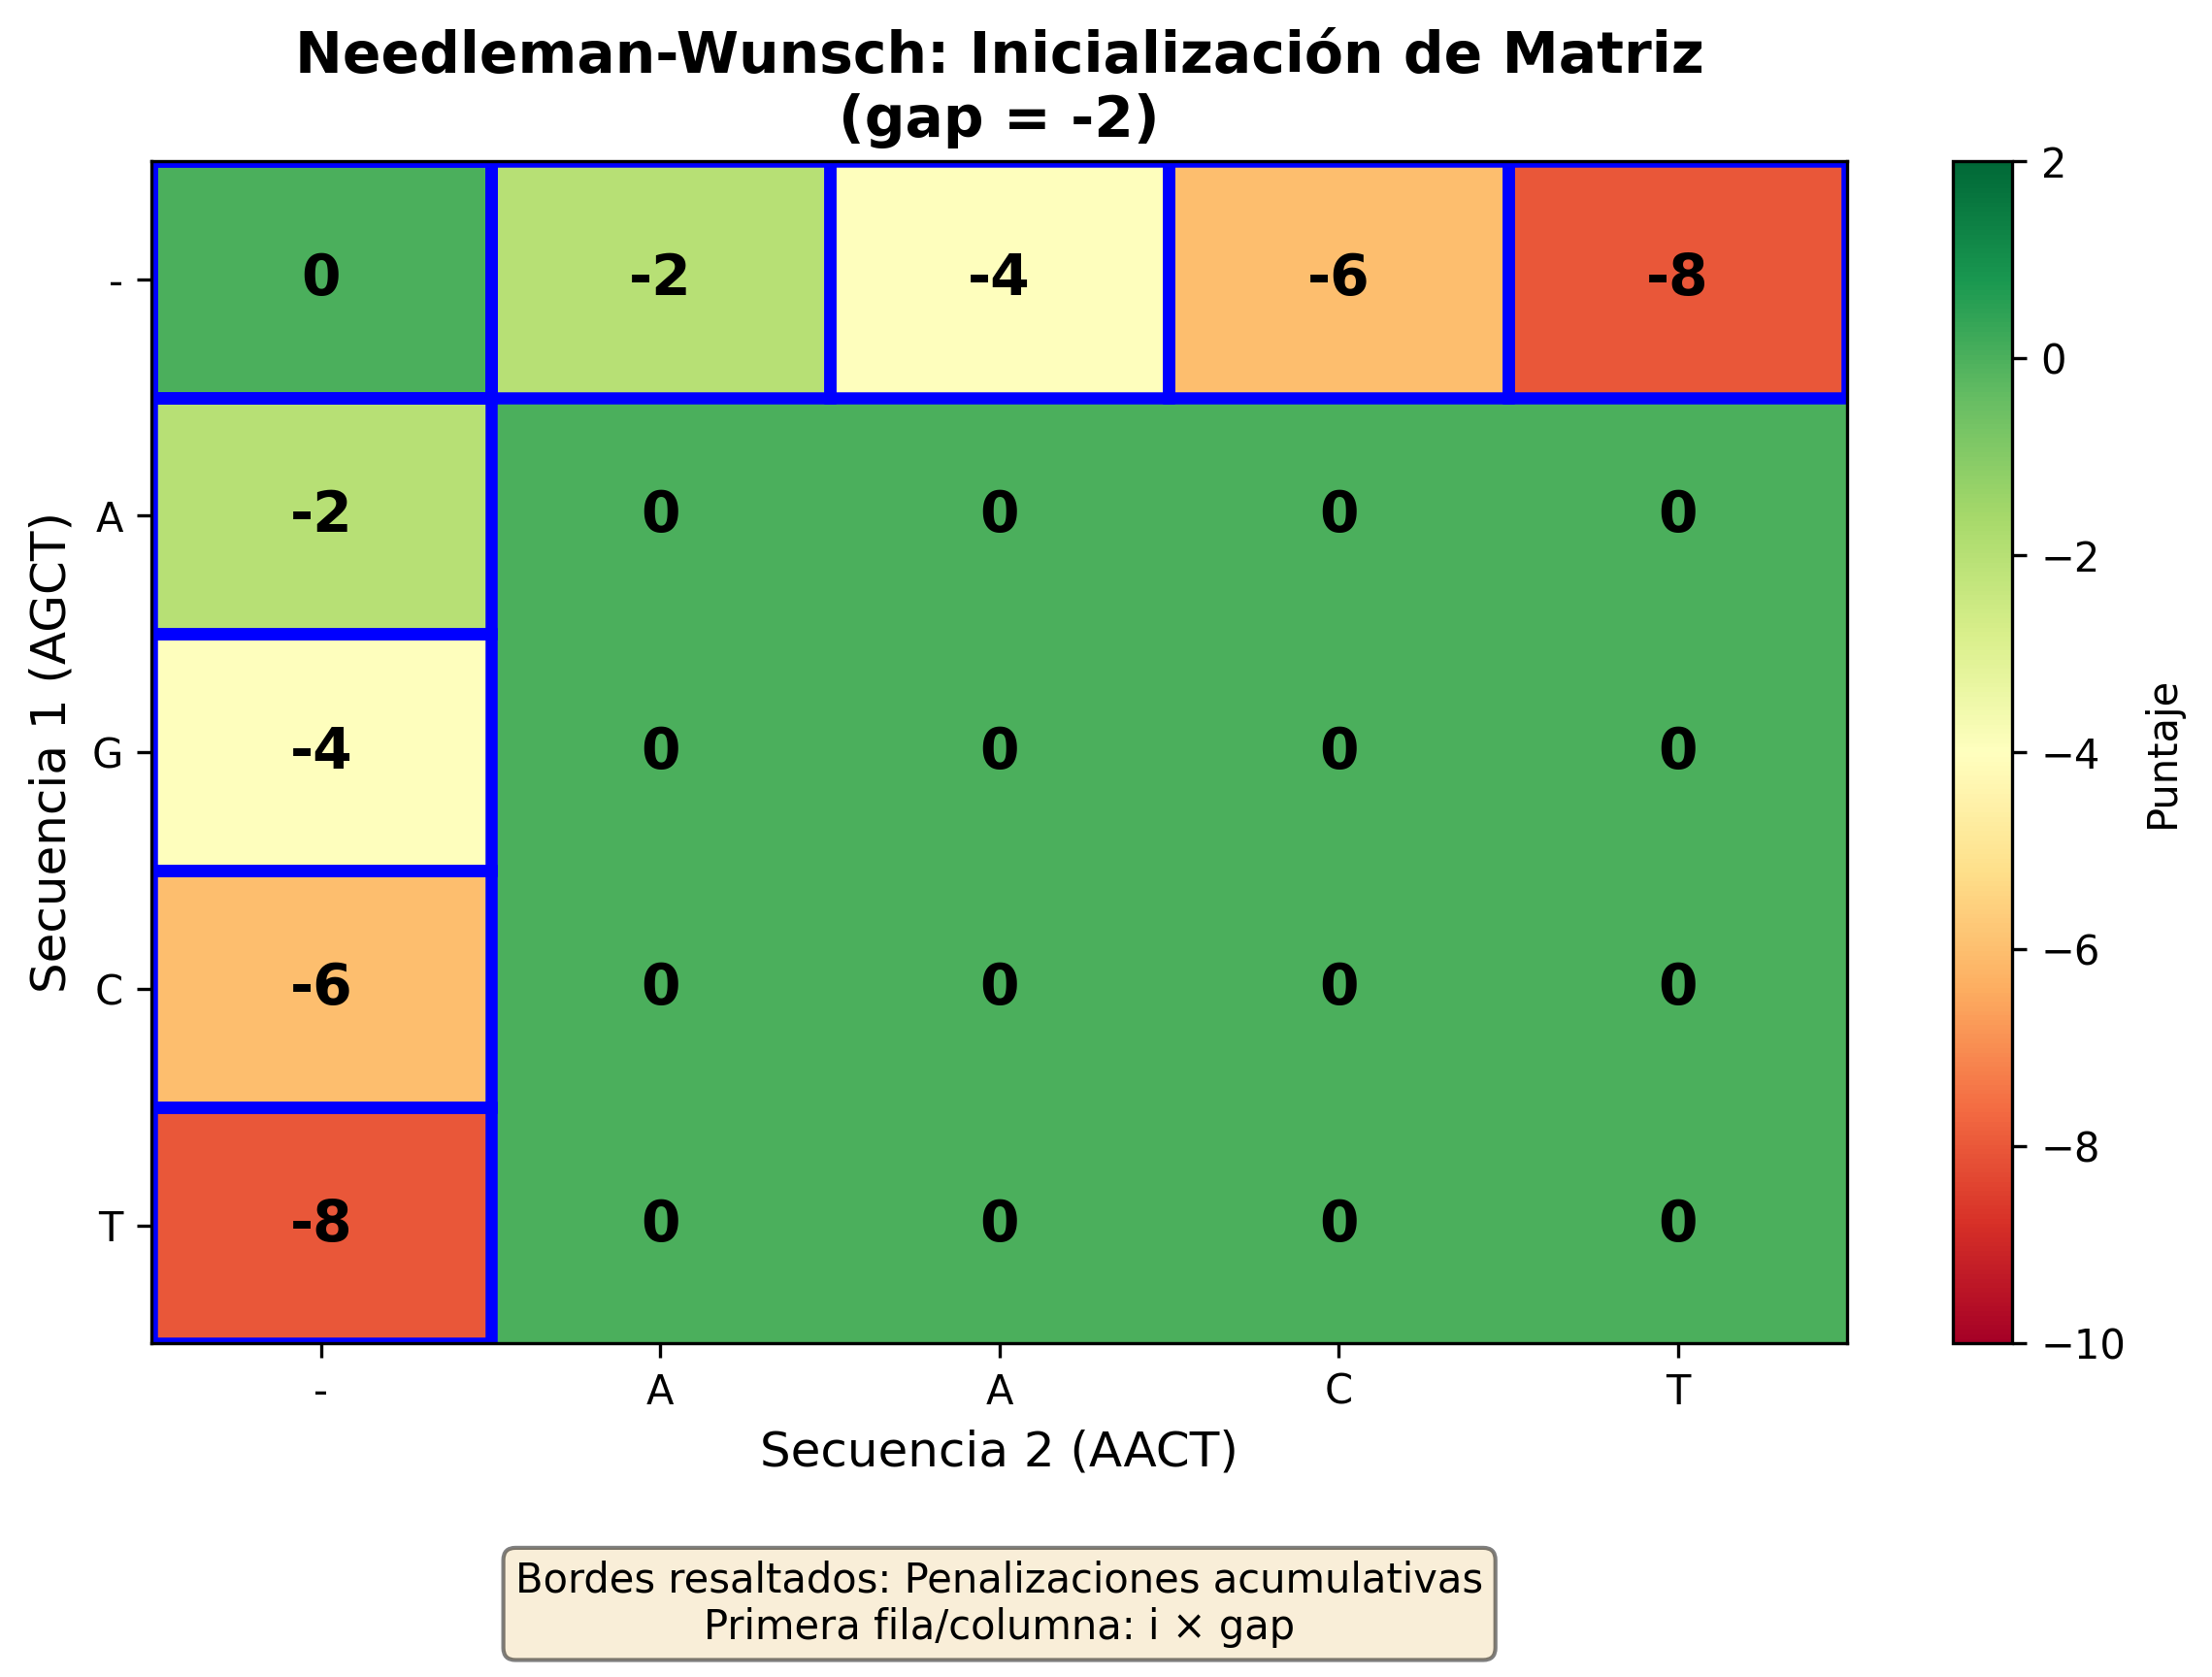
\includegraphics[width=0.6\textwidth]{img/nw_initialization.png}
\caption{Inicialización de la matriz en Needleman-Wunsch}
\label{fig:nw_init}
\end{figure}

\textbf{2. Llenado de la Matriz (Programación Dinámica)}

Para cada celda $M[i][j]$, se calcula:

\begin{equation}
M[i][j] = \max \begin{cases}
M[i-1][j-1] + s(a_i, b_j) & \text{(diagonal: match/mismatch)} \\
M[i-1][j] + s_{\text{gap}} & \text{(arriba: gap en secuencia 2)} \\
M[i][j-1] + s_{\text{gap}} & \text{(izquierda: gap en secuencia 1)}
\end{cases}
\end{equation}

Donde $s(a_i, b_j)$ es:
\begin{equation}
s(a_i, b_j) = \begin{cases}
s_{\text{match}} & \text{si } a_i = b_j \\
s_{\text{mismatch}} & \text{si } a_i \neq b_j
\end{cases}
\end{equation}

\begin{figure}[H]
\centering
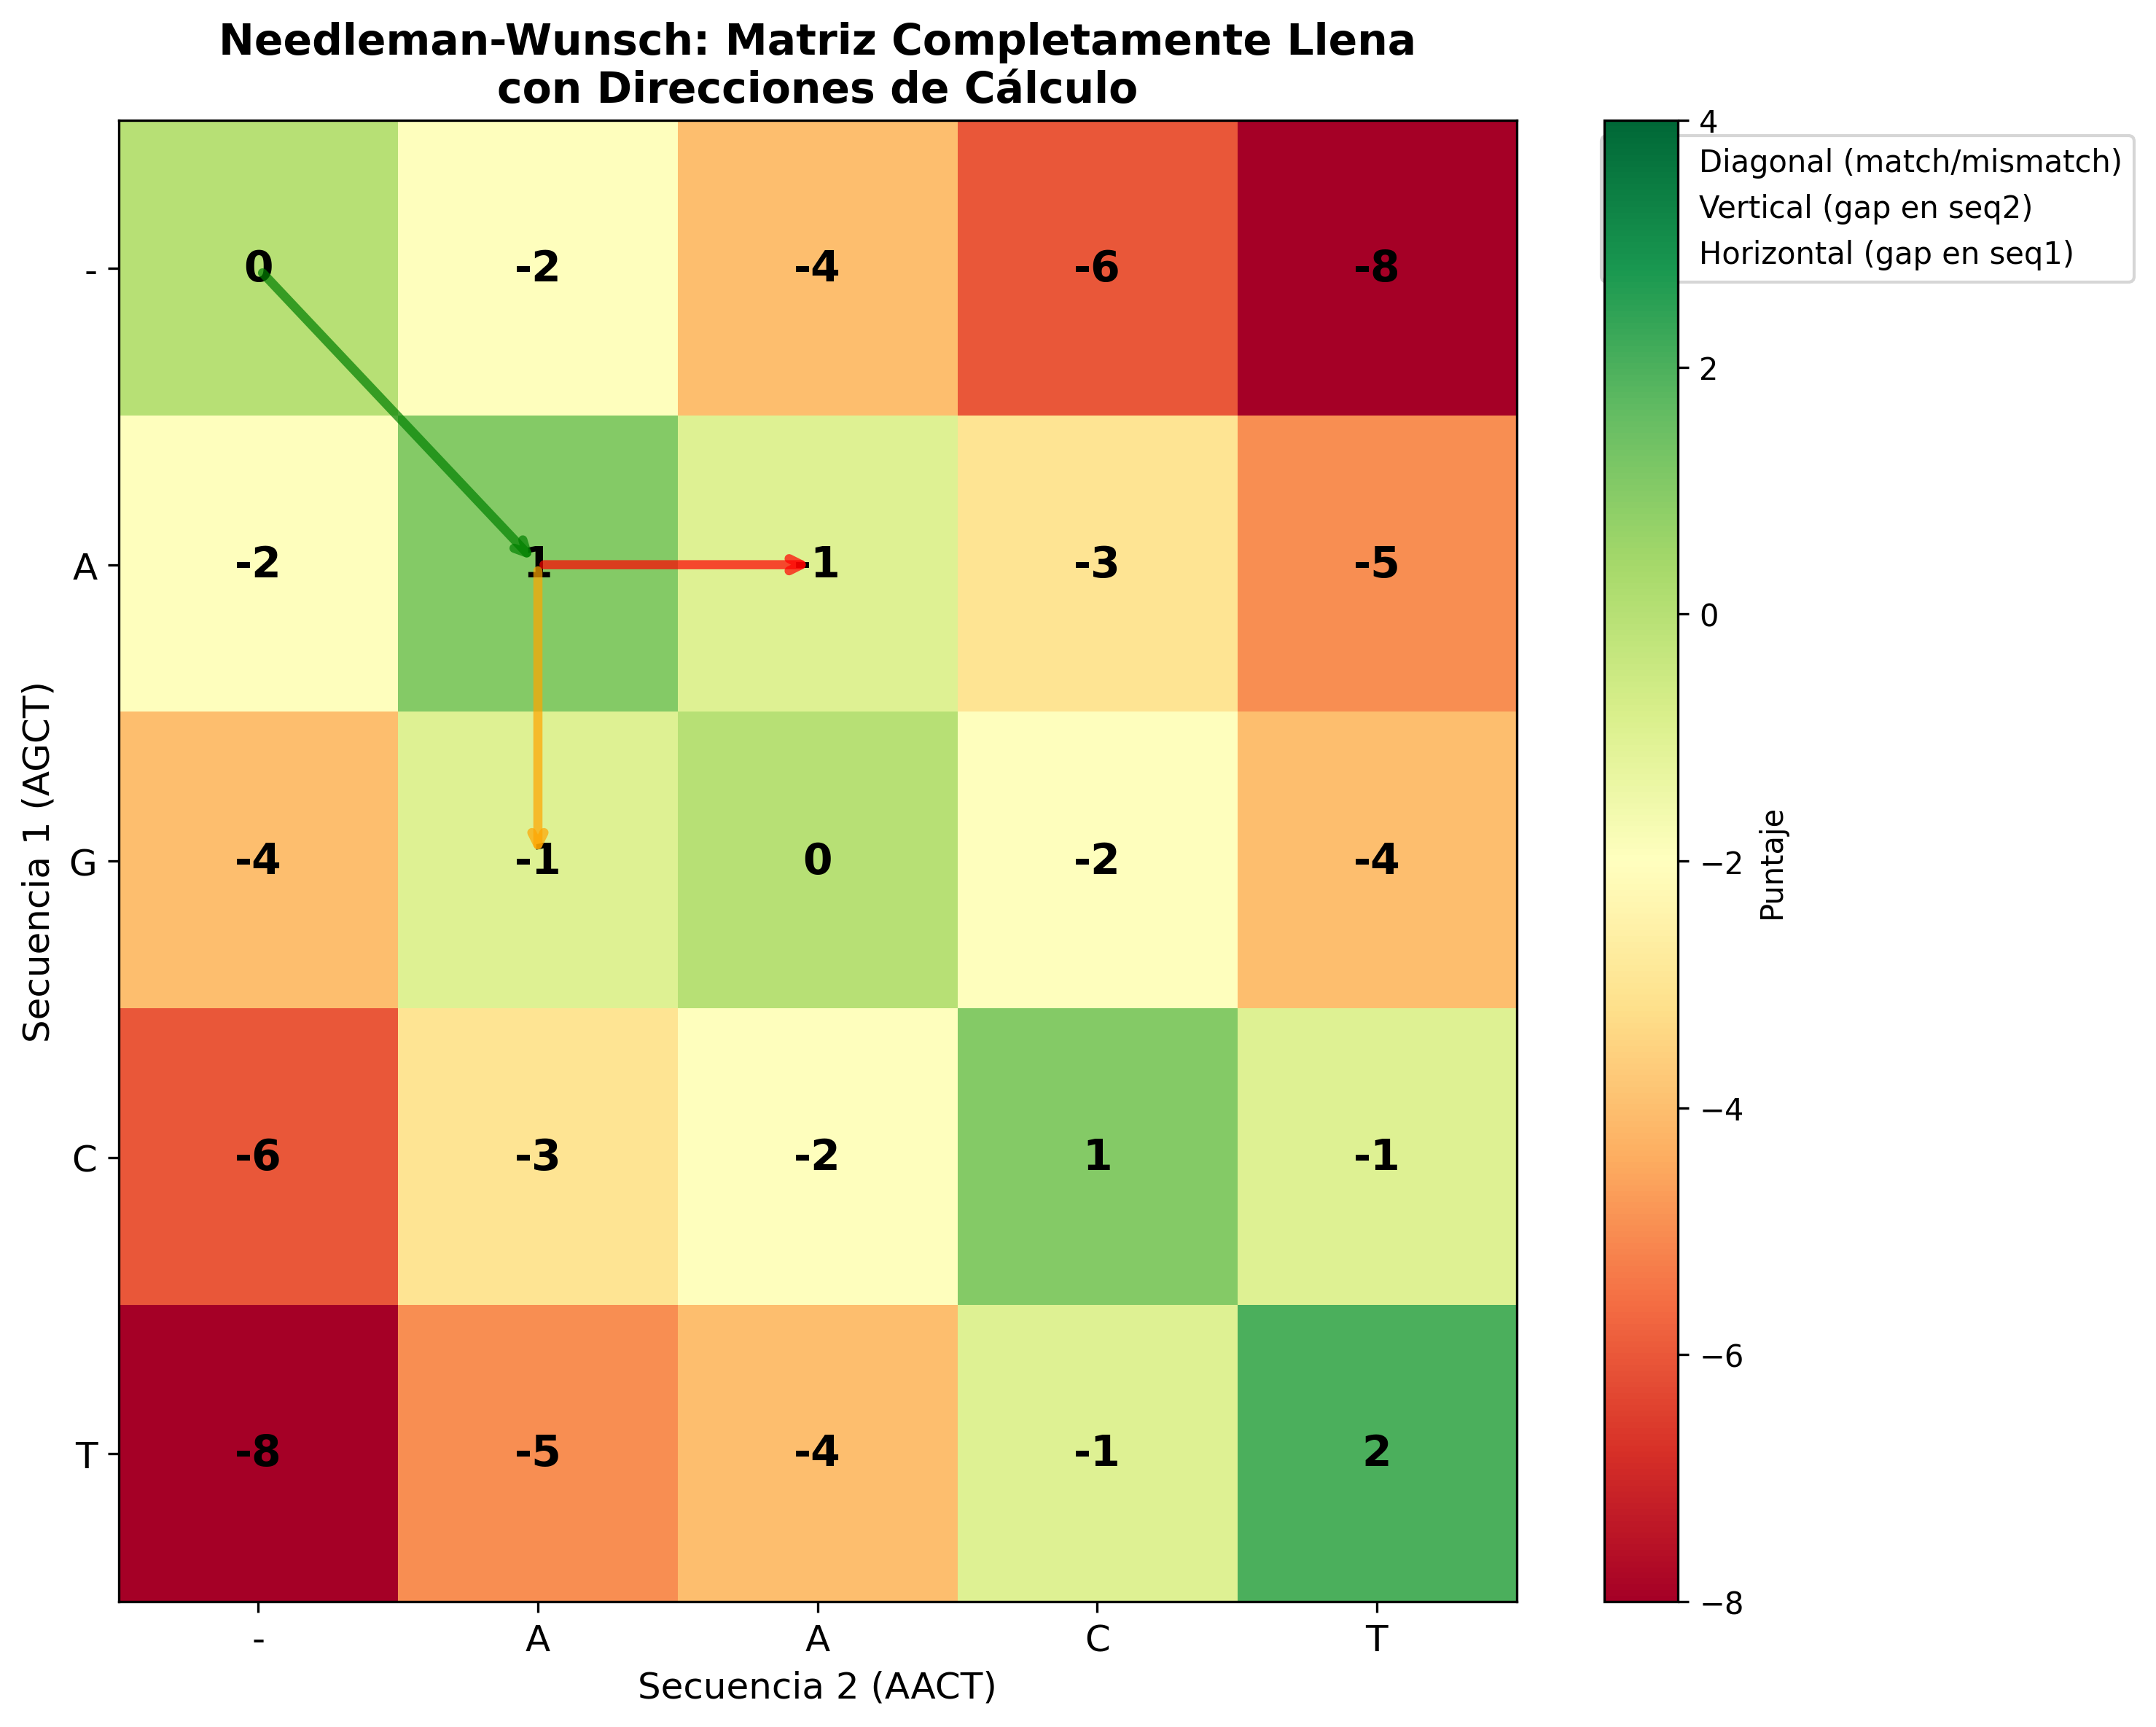
\includegraphics[width=0.7\textwidth]{img/nw_filling.png}
\caption{Proceso de llenado de la matriz en Needleman-Wunsch}
\label{fig:nw_fill}
\end{figure}

\textbf{3. Traceback (Reconstrucción del Alineamiento)}

Comenzando desde $M[m][n]$, se sigue el camino que generó los valores máximos:

\begin{itemize}
    \item Si vino de la diagonal: alinear $a_i$ con $b_j$
    \item Si vino de arriba: insertar gap en secuencia 2 (alinear $a_i$ con -)
    \item Si vino de izquierda: insertar gap en secuencia 1 (alinear - con $b_j$)
\end{itemize}

El proceso termina al llegar a $M[0][0]$.

\begin{figure}[H]
\centering
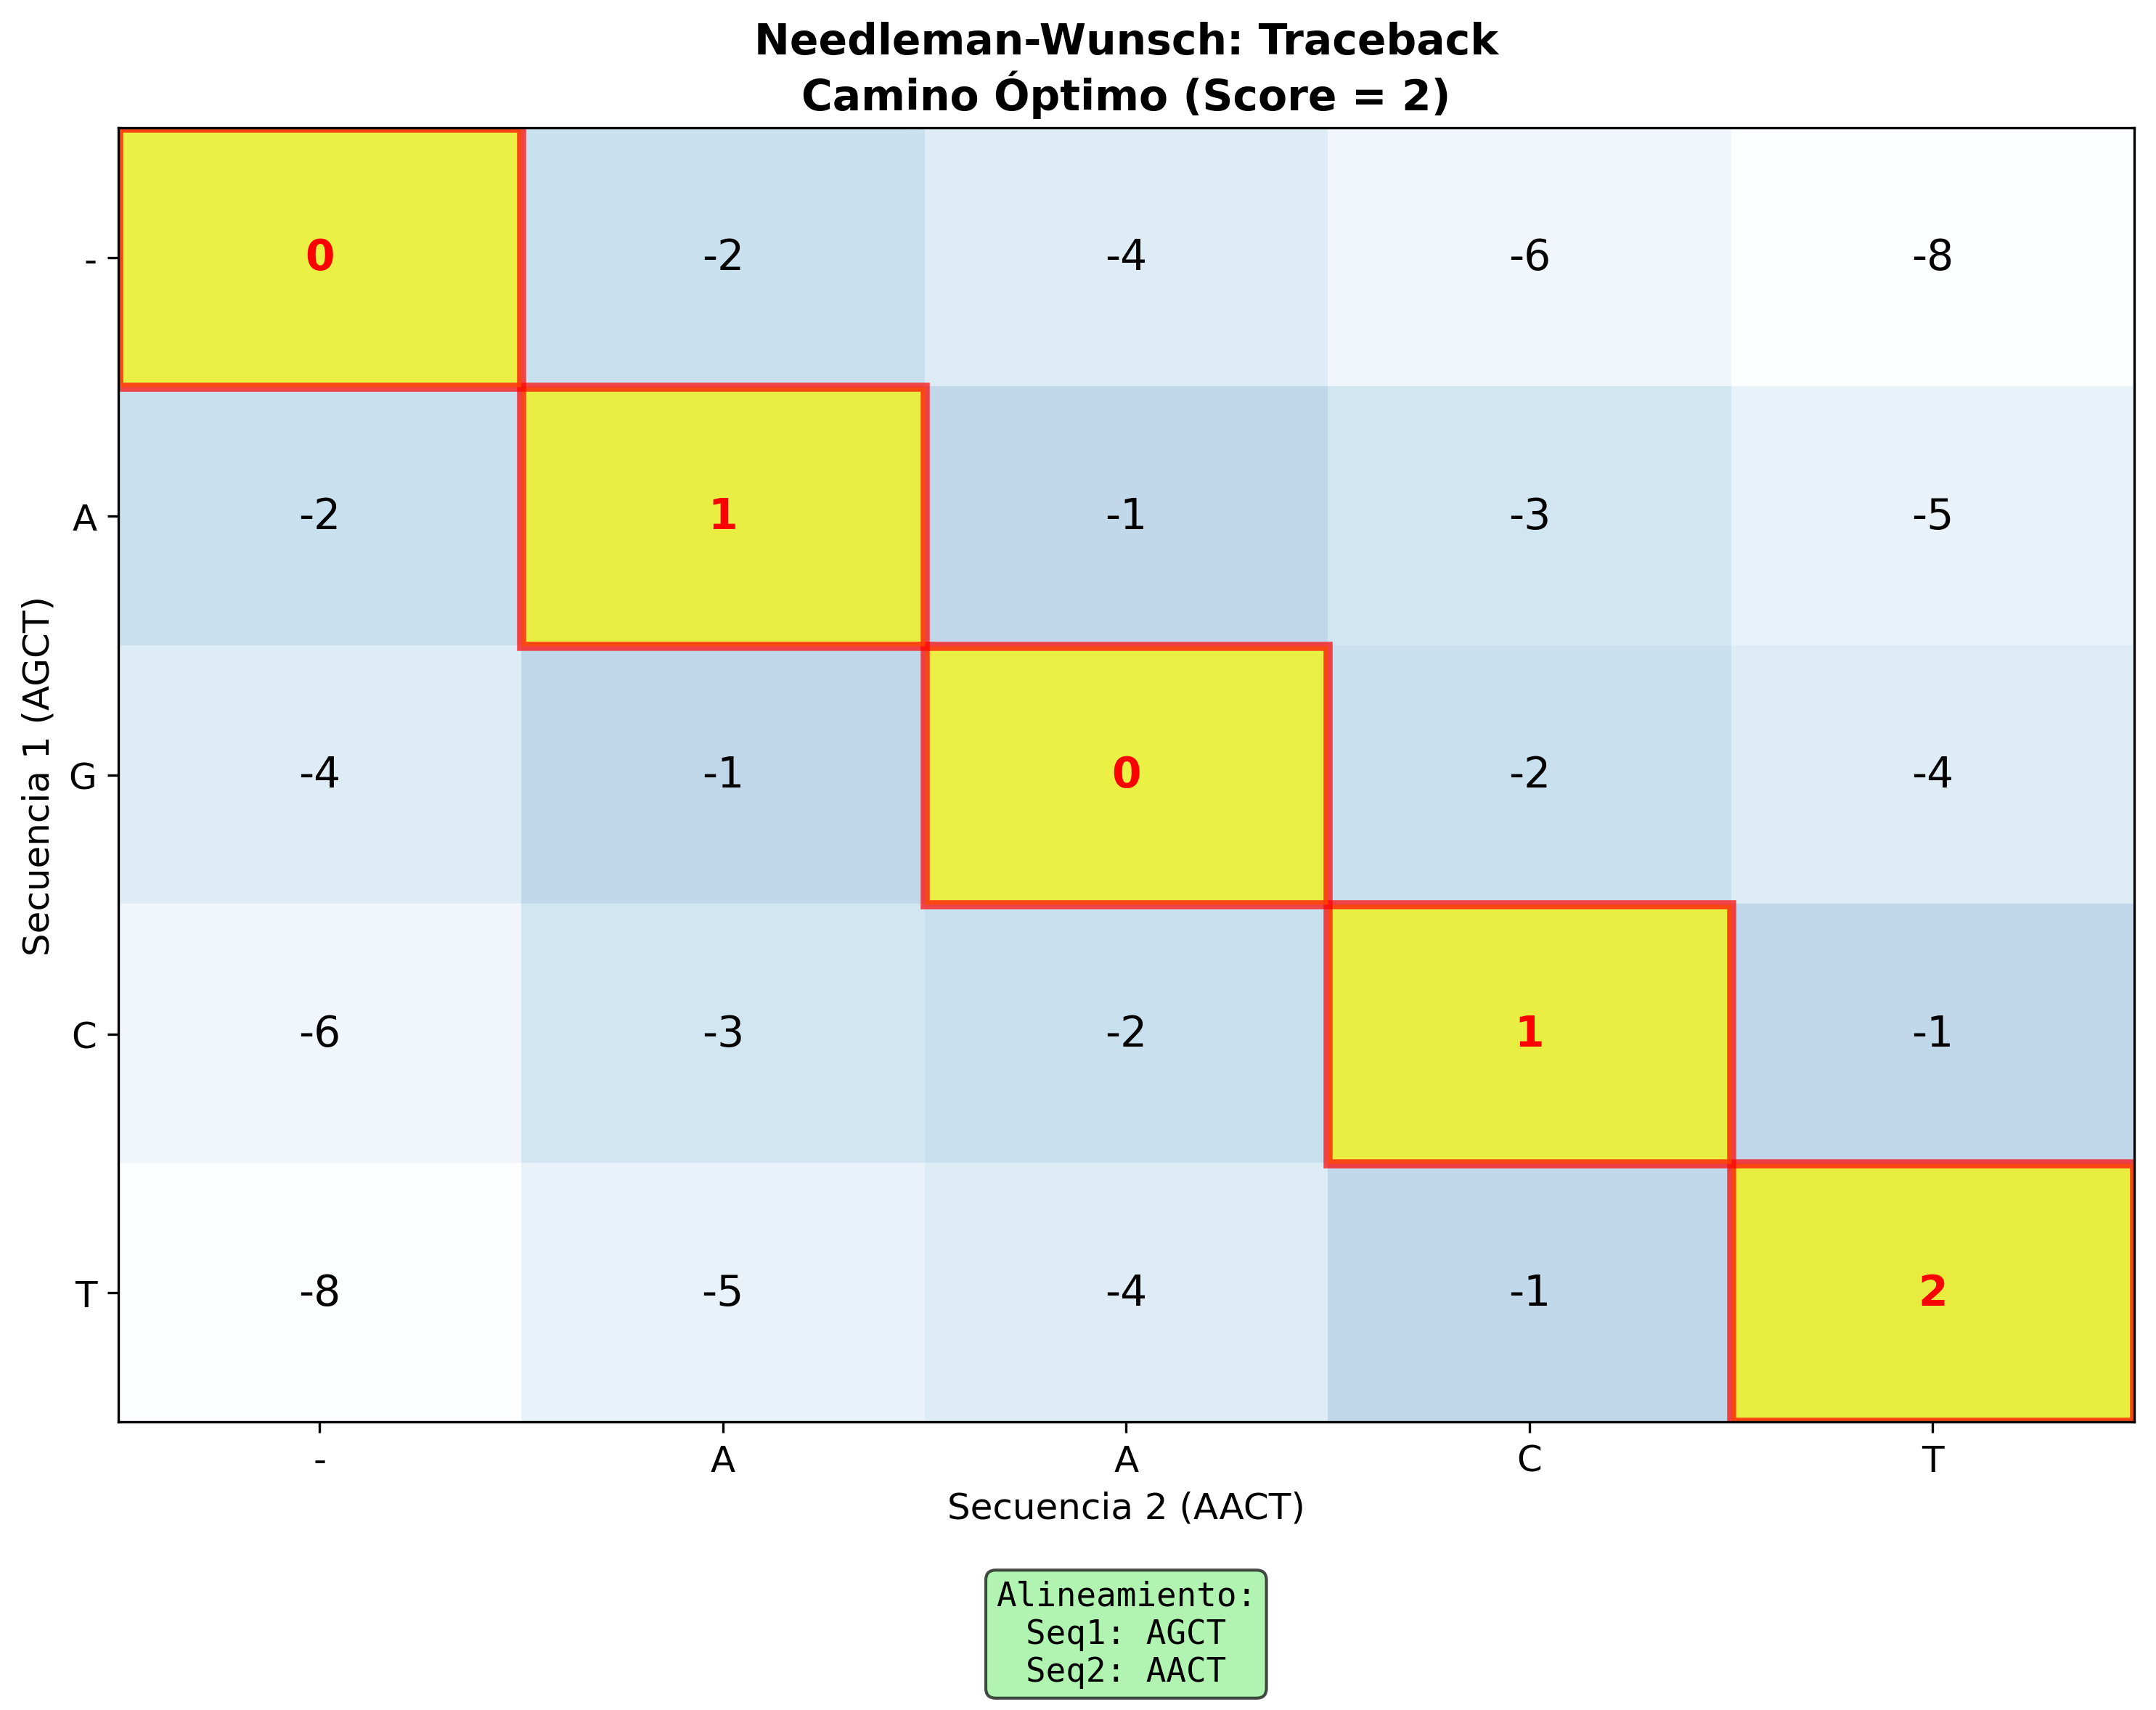
\includegraphics[width=0.7\textwidth]{img/nw_traceback.png}
\caption{Traceback en Needleman-Wunsch para reconstruir el alineamiento}
\label{fig:nw_traceback}
\end{figure}

\subsubsection{Implementación en Python}

\begin{lstlisting}[language=Python, caption=Clase NeedlemanWunsch en Python]
class NeedlemanWunsch:
    def __init__(self, match=1, mismatch=-1, gap=-2):
        """Inicializa los parametros de puntuacion"""
        self.match = match
        self.mismatch = mismatch
        self.gap = gap
    
    def calculate_score(self, a, b):
        """Calcula puntuacion entre dos caracteres"""
        return self.match if a == b else self.mismatch
    
    def initialize_matrix(self, seq1, seq2):
        """Inicializa matriz con penalizaciones acumulativas"""
        rows = len(seq1) + 1
        cols = len(seq2) + 1
        
        matrix = [[0 for _ in range(cols)] for _ in range(rows)]
        
        # Primera columna
        for i in range(rows):
            matrix[i][0] = i * self.gap
        
        # Primera fila
        for j in range(cols):
            matrix[0][j] = j * self.gap
        
        return matrix
    
    def fill_matrix(self, matrix, seq1, seq2):
        """Llena la matriz usando programacion dinamica"""
        for i in range(1, len(seq1) + 1):
            for j in range(1, len(seq2) + 1):
                # Calcular puntaje diagonal (match/mismatch)
                match_score = matrix[i-1][j-1] + \
                             self.calculate_score(seq1[i-1], seq2[j-1])
                
                # Calcular puntaje vertical (gap en seq2)
                gap_vertical = matrix[i-1][j] + self.gap
                
                # Calcular puntaje horizontal (gap en seq1)
                gap_horizontal = matrix[i][j-1] + self.gap
                
                # Tomar el maximo
                matrix[i][j] = max(match_score, gap_vertical, gap_horizontal)
        
        return matrix
    
    def traceback(self, seq1, seq2, matrix):
        """Reconstruye el alineamiento desde (m,n) hasta (0,0)"""
        aligned1 = []
        aligned2 = []
        i = len(seq1)
        j = len(seq2)
        
        while i > 0 or j > 0:
            if i > 0 and j == 0:
                aligned1.append(seq1[i-1])
                aligned2.append('-')
                i -= 1
            elif i == 0 and j > 0:
                aligned1.append('-')
                aligned2.append(seq2[j-1])
                j -= 1
            else:
                current_score = matrix[i][j]
                diagonal_score = matrix[i-1][j-1] + \
                                self.calculate_score(seq1[i-1], seq2[j-1])
                up_score = matrix[i-1][j] + self.gap
                left_score = matrix[i][j-1] + self.gap
                
                if current_score == diagonal_score:
                    aligned1.append(seq1[i-1])
                    aligned2.append(seq2[j-1])
                    i -= 1
                    j -= 1
                elif current_score == up_score:
                    aligned1.append(seq1[i-1])
                    aligned2.append('-')
                    i -= 1
                else:
                    aligned1.append('-')
                    aligned2.append(seq2[j-1])
                    j -= 1
        
        return ''.join(reversed(aligned1)), ''.join(reversed(aligned2))
    
    def alignment(self, seq1, seq2):
        """Ejecuta el algoritmo completo"""
        matrix = self.initialize_matrix(seq1, seq2)
        matrix = self.fill_matrix(matrix, seq1, seq2)
        aligned1, aligned2 = self.traceback(seq1, seq2, matrix)
        score = matrix[len(seq1)][len(seq2)]
        
        return aligned1, aligned2, score, matrix
\end{lstlisting}

\subsection{Smith-Waterman: Alineamiento Local}

\subsubsection{Descripción del Algoritmo}

El algoritmo de Smith-Waterman (1981) es una variante del algoritmo de Needleman-Wunsch diseñada para encontrar el mejor alineamiento local entre dos secuencias. Es particularmente útil para identificar regiones conservadas o dominios funcionales.

\subsubsection{Diferencias con Needleman-Wunsch}

\begin{table}[H]
\centering
\caption{Comparación entre Needleman-Wunsch y Smith-Waterman}
\begin{tabular}{@{}lll@{}}
\toprule
\textbf{Aspecto} & \textbf{Needleman-Wunsch} & \textbf{Smith-Waterman} \\ \midrule
Tipo & Alineamiento global & Alineamiento local \\
Inicialización & Penalizaciones acumulativas & Todo en ceros \\
Llenado & max(diagonal, arriba, izq) & max(diagonal, arriba, izq, \textbf{0}) \\
Inicio traceback & Celda $(m,n)$ & Celda con \textbf{valor máximo} \\
Fin traceback & Celda $(0,0)$ & Primera celda con \textbf{valor 0} \\
Aplicación & Genes ortólogos & Dominios conservados \\ \bottomrule
\end{tabular}
\label{tab:nw_vs_sw}
\end{table}

\subsubsection{Fases del Algoritmo}

\textbf{1. Inicialización}

\begin{align}
M[i][0] &= 0 \quad \text{para } i = 0 \ldots m \\
M[0][j] &= 0 \quad \text{para } j = 0 \ldots n
\end{align}

\textbf{2. Llenado de la Matriz}

\begin{equation}
M[i][j] = \max \begin{cases}
0 & \text{(reiniciar - diferencia clave)} \\
M[i-1][j-1] + s(a_i, b_j) & \text{(diagonal)} \\
M[i-1][j] + s_{\text{gap}} & \text{(arriba)} \\
M[i][j-1] + s_{\text{gap}} & \text{(izquierda)}
\end{cases}
\end{equation}

\begin{figure}[H]
\centering
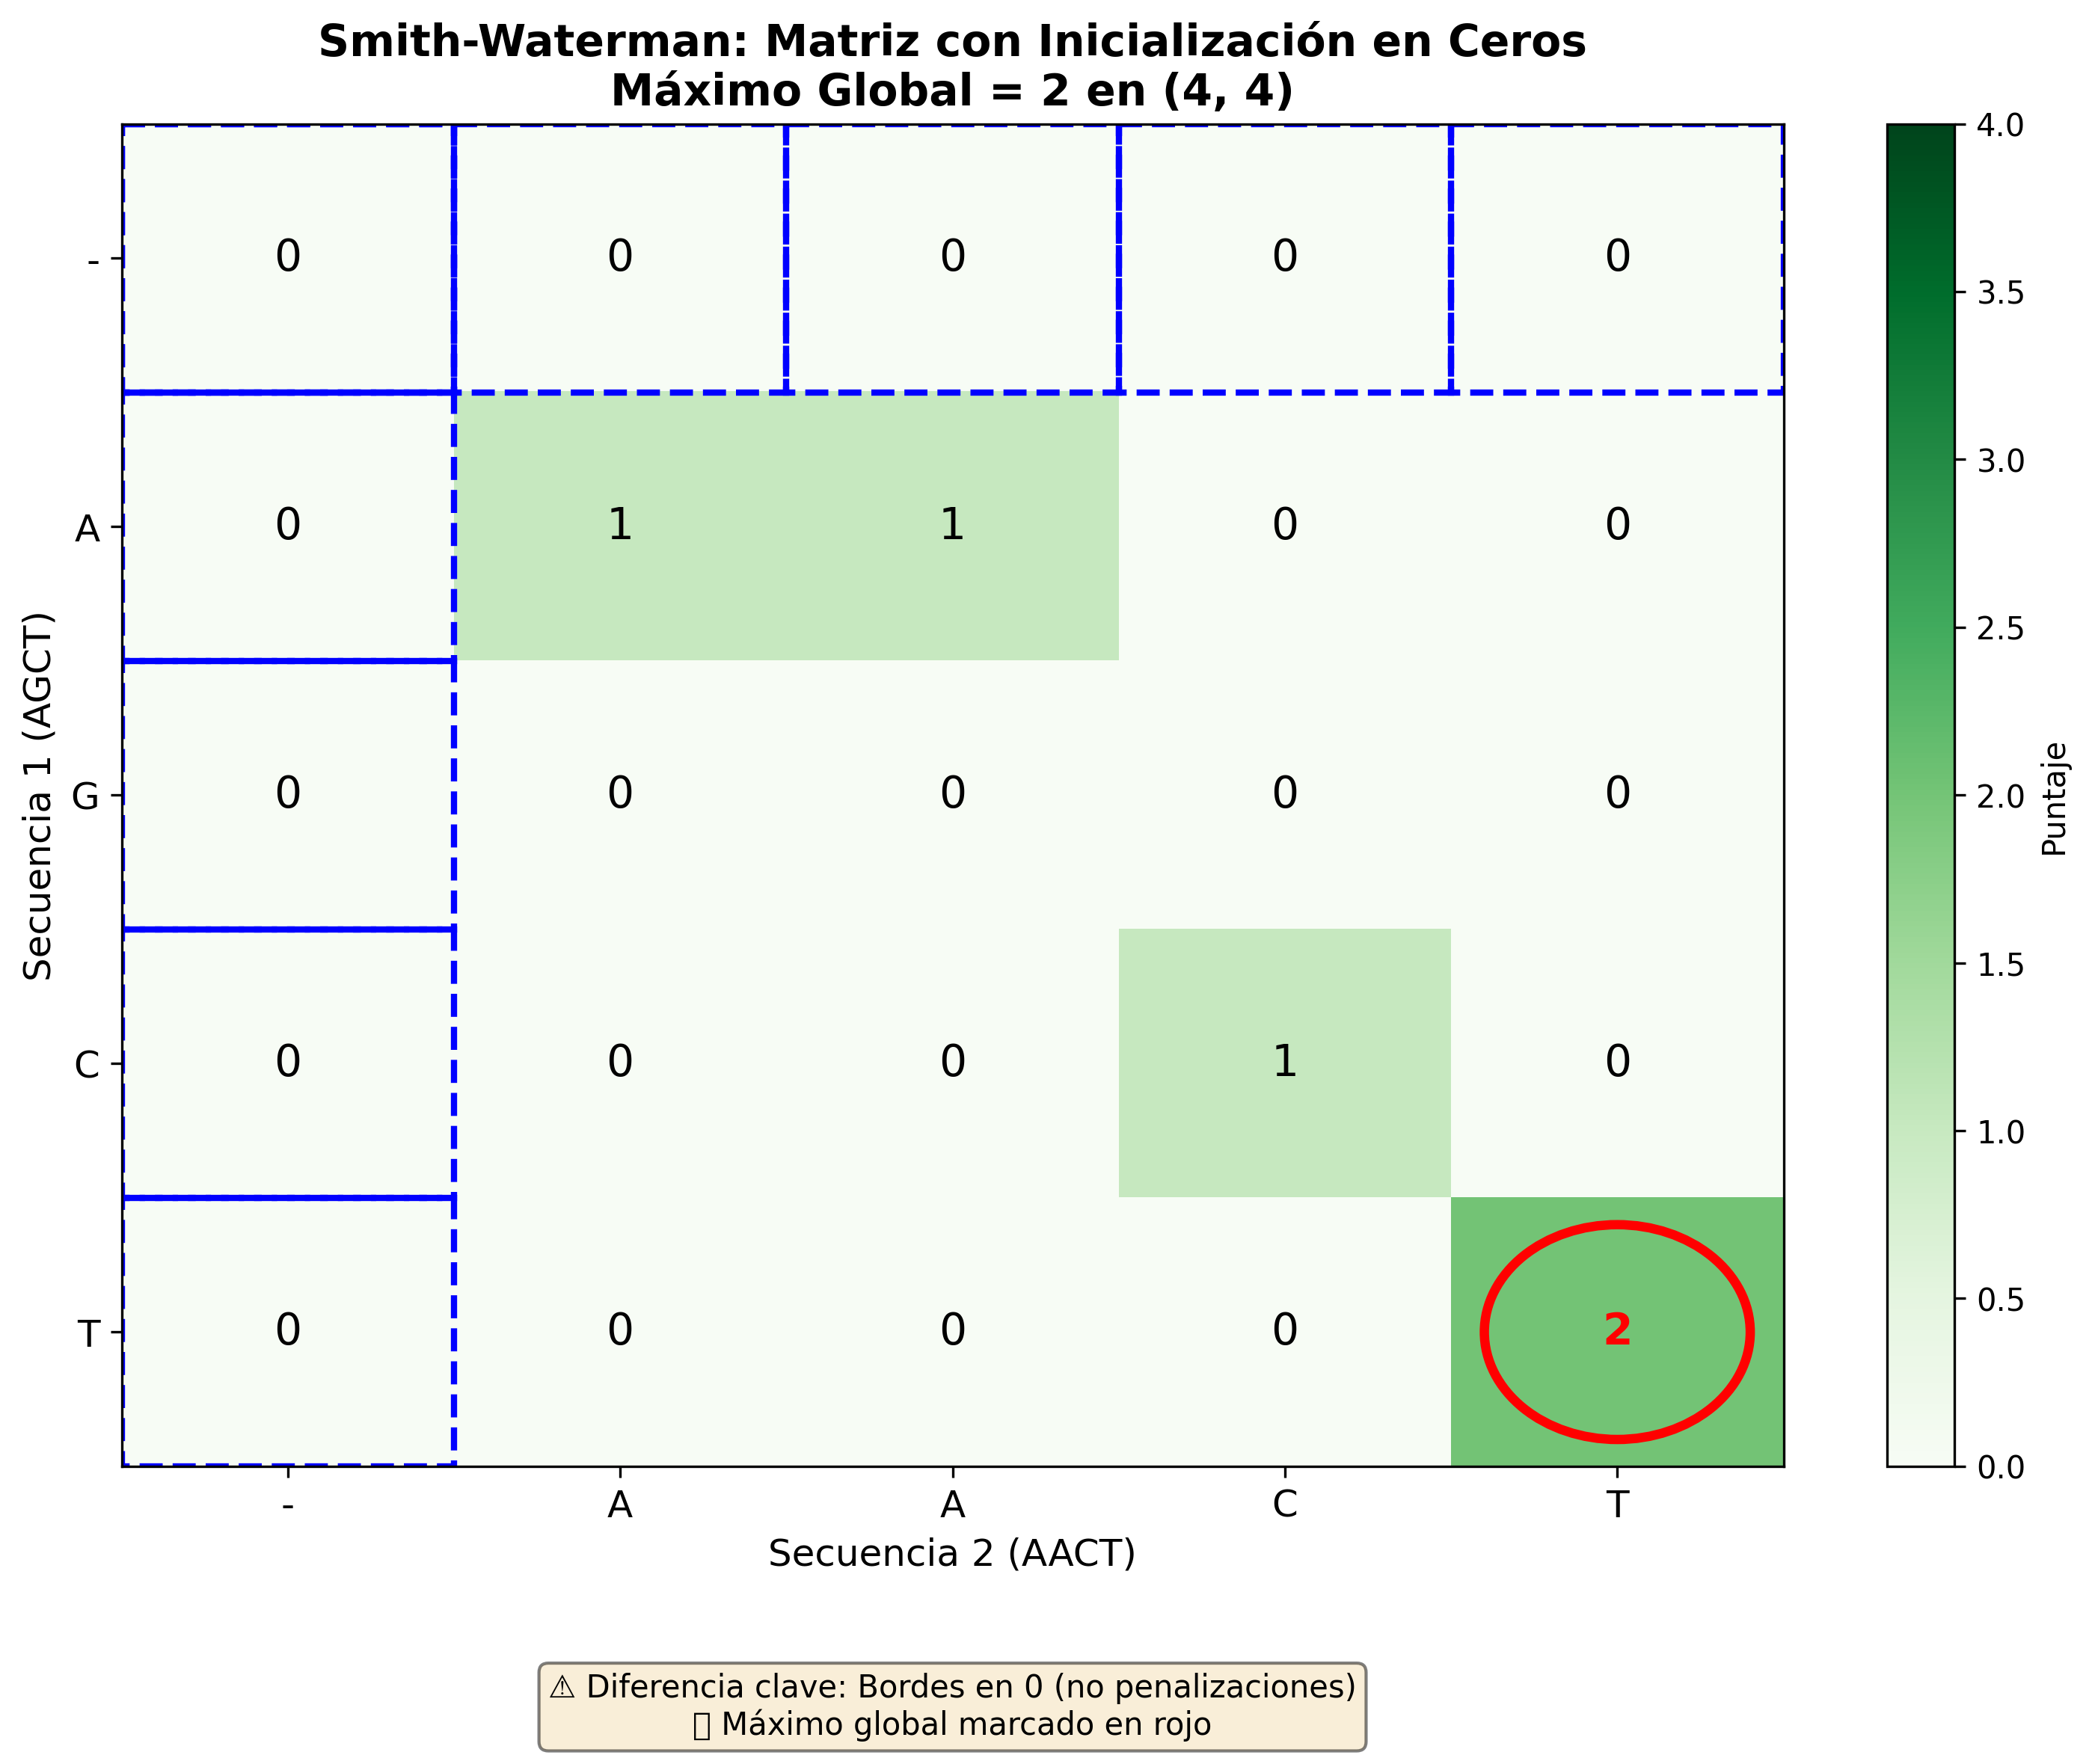
\includegraphics[width=0.7\textwidth]{img/sw_matrix.png}
\caption{Matriz de Smith-Waterman con valores no negativos}
\label{fig:sw_matrix}
\end{figure}

\textbf{3. Traceback}

\begin{enumerate}
    \item Encontrar el valor máximo en toda la matriz: $M_{\max} = M[i_{\max}][j_{\max}]$
    \item Iniciar traceback desde $(i_{\max}, j_{\max})$
    \item Continuar hasta encontrar una celda con valor 0
\end{enumerate}

\begin{figure}[H]
\centering
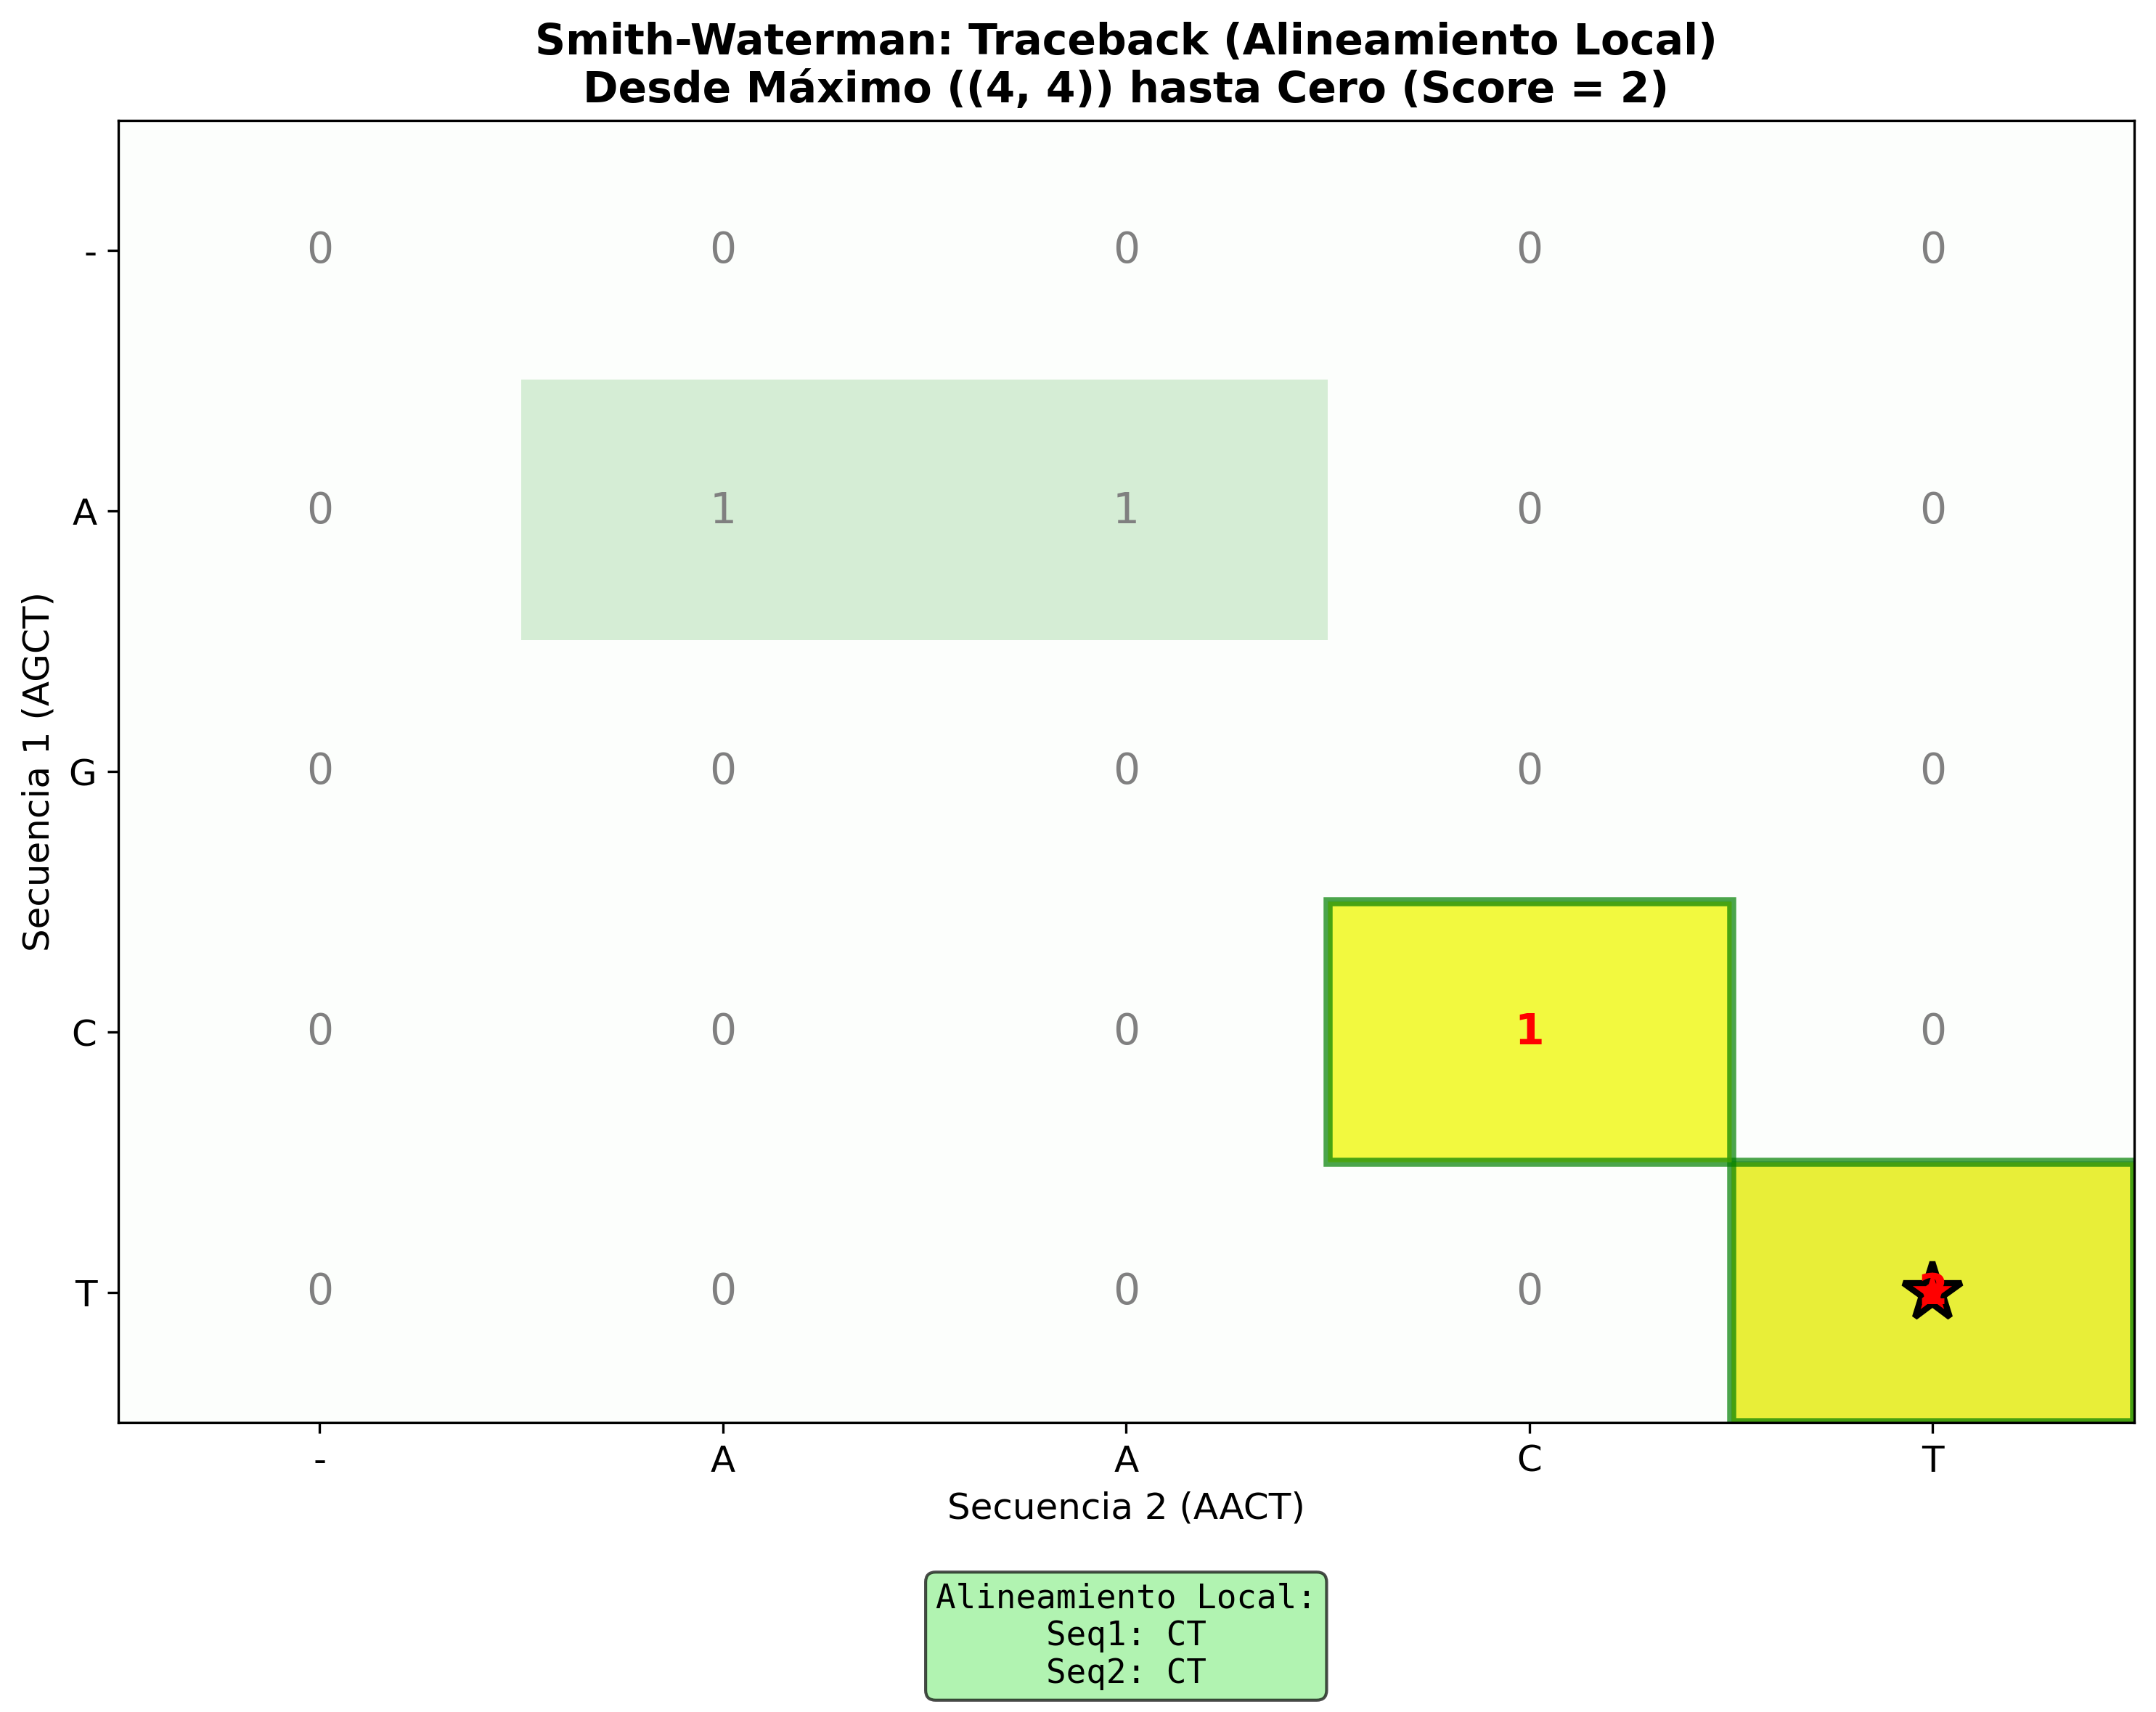
\includegraphics[width=0.7\textwidth]{img/sw_traceback.png}
\caption{Traceback en Smith-Waterman desde el máximo hasta cero}
\label{fig:sw_traceback}
\end{figure}

\subsubsection{Implementación en Python}

\begin{lstlisting}[language=Python, caption=Clase SmithWaterman en Python]
class SmithWaterman:
    def __init__(self, match=1, mismatch=-1, gap=-2):
        """Inicializa los parametros de puntuacion"""
        self.match = match
        self.mismatch = mismatch
        self.gap = gap
    
    def calculate_score(self, a, b):
        """Calcula puntuacion entre dos caracteres"""
        return self.match if a == b else self.mismatch
    
    def initialize_matrix(self, seq1, seq2):
        """Inicializa matriz con ceros (diferencia clave con NW)"""
        rows = len(seq1) + 1
        cols = len(seq2) + 1
        
        # Toda la matriz en ceros
        matrix = [[0 for _ in range(cols)] for _ in range(rows)]
        
        return matrix
    
    def fill_matrix(self, matrix, seq1, seq2):
        """Llena la matriz usando programacion dinamica"""
        for i in range(1, len(seq1) + 1):
            for j in range(1, len(seq2) + 1):
                # Calcular puntaje diagonal (match/mismatch)
                match_score = matrix[i-1][j-1] + \
                             self.calculate_score(seq1[i-1], seq2[j-1])
                
                # Calcular puntaje vertical (gap en seq2)
                gap_vertical = matrix[i-1][j] + self.gap
                
                # Calcular puntaje horizontal (gap en seq1)
                gap_horizontal = matrix[i][j-1] + self.gap
                
                # DIFERENCIA CLAVE: incluir 0 en el maximo
                matrix[i][j] = max(0, match_score, gap_vertical, 
                                  gap_horizontal)
        
        return matrix
    
    def find_max(self, matrix):
        """Encuentra la posicion del valor maximo en la matriz"""
        max_score = 0
        max_pos = (0, 0)
        
        for i in range(len(matrix)):
            for j in range(len(matrix[0])):
                if matrix[i][j] > max_score:
                    max_score = matrix[i][j]
                    max_pos = (i, j)
        
        return max_pos, max_score
    
    def traceback(self, seq1, seq2, matrix, start_pos):
        """Reconstruye alineamiento desde maximo hasta encontrar 0"""
        aligned1 = []
        aligned2 = []
        i, j = start_pos
        
        # Continuar mientras no se llegue a 0
        while i > 0 and j > 0 and matrix[i][j] > 0:
            current_score = matrix[i][j]
            diagonal_score = matrix[i-1][j-1] + \
                            self.calculate_score(seq1[i-1], seq2[j-1])
            up_score = matrix[i-1][j] + self.gap
            left_score = matrix[i][j-1] + self.gap
            
            if current_score == diagonal_score:
                aligned1.append(seq1[i-1])
                aligned2.append(seq2[j-1])
                i -= 1
                j -= 1
            elif current_score == up_score:
                aligned1.append(seq1[i-1])
                aligned2.append('-')
                i -= 1
            else:
                aligned1.append('-')
                aligned2.append(seq2[j-1])
                j -= 1
        
        return ''.join(reversed(aligned1)), ''.join(reversed(aligned2))
    
    def alignment(self, seq1, seq2):
        """Ejecuta el algoritmo completo"""
        matrix = self.initialize_matrix(seq1, seq2)
        matrix = self.fill_matrix(matrix, seq1, seq2)
        max_pos, score = self.find_max(matrix)
        aligned1, aligned2 = self.traceback(seq1, seq2, matrix, max_pos)
        
        return aligned1, aligned2, score, matrix
\end{lstlisting}

% -------------------------
% CASOS DE PRUEBA
% -------------------------
\subsection{Casos de Prueba Implementados}

\begin{table}[H]
\centering
\caption{Suite de tests implementada}
\begin{tabular}{@{}lp{8cm}@{}}
\toprule
\textbf{Test} & \textbf{Descripción} \\ \midrule
test\_simple.py & Demostración con secuencias cortas (7 caracteres) \\
test\_hemoglobin.py & Hemoglobina: Homo Sapiens vs Conejo (142 aa) \\
test\_insulin.py & Insulina: Homo Sapiens vs Gorila (1431 vs 978 aa) \\
test\_special.py & Casos especiales (idénticas, sin similitud, subsecuencias) \\ \bottomrule
\end{tabular}
\label{tab:tests}
\end{table}

% -------------------------
% RESULTADOS
% -------------------------
\section{Resultados Experimentales}

\subsection{Caso 1: Hemoglobina - Homo Sapiens vs Conejo}

\textbf{Secuencias:} 142 aminoácidos (ambas especies)

\begin{table}[H]
\centering
\caption{Resultados hemoglobina}
\begin{tabular}{@{}lcc@{}}
\toprule
\textbf{Métrica} & \textbf{NW} & \textbf{SW} \\ \midrule
Puntuación & 92 & 92 \\
Identidad & 82.4\% & 82.4\% \\
Matches & 117 & 117 \\
Gaps & 0 & 0 \\ \bottomrule
\end{tabular}
\end{table}

\textbf{Interpretación:} Alta conservación funcional (82.4\%) refleja la importancia crítica de la hemoglobina en el transporte de oxígeno. Los resultados idénticos entre NW y SW indican que la similitud es uniforme a lo largo de toda la secuencia.

\subsection{Caso 2: Insulina - Homo Sapiens vs Gorila}

\textbf{Secuencias:} 1431 aminoácidos (Homo Sapiens) vs 978 aminoácidos (Gorila)

\begin{table}[H]
\centering
\caption{Resultados insulina}
\begin{tabular}{@{}lcc@{}}
\toprule
\textbf{Métrica} & \textbf{NW} & \textbf{SW} \\ \midrule
Puntuación & 5 & 895 \\
Identidad & 66.3\% & 96.1\% \\
Matches & 952 & 949 \\
Gaps & 463 & 15 \\ \bottomrule
\end{tabular}
\end{table}

\textbf{Interpretación:} La gran diferencia entre NW y SW revela la naturaleza de las secuencias. NW (66.3\%) penaliza fuertemente la diferencia de longitud con 463 gaps. SW (96.1\%) identifica la región funcional conservada de la insulina con alta identidad, demostrando la utilidad del alineamiento local para secuencias de longitud diferente.

% -------------------------
% CONCLUSIONES
% -------------------------
\section{Conclusiones}

\begin{enumerate}
    \item Se implementaron exitosamente los algoritmos de Needleman-Wunsch y Smith-Waterman en Python con arquitectura modular.
    
    \item Los resultados experimentales validaron la correctitud de la implementación con secuencias biológicas reales.
    
    \item Para secuencias de longitud similar y alta similitud (hemoglobina), ambos algoritmos convergen al mismo resultado (82.4\% identidad).
    
    \item Para secuencias de longitud muy diferente (insulina), Smith-Waterman es superior al identificar la región conservada con 96.1\% de identidad, mientras que Needleman-Wunsch solo alcanza 66.3\% por la penalización de 463 gaps.
    
    \item La visualización y exportación de resultados facilita la interpretación de alineamientos largos (>1000 caracteres).
\end{enumerate}

\textbf{Trabajo futuro:} Implementar matrices BLOSUM/PAM, penalizaciones affine para gaps, optimización con Hirschberg para reducir complejidad espacial.

\vspace{1cm}

% -------------------------
% REFERENCIAS (OPCIONAL)
% -------------------------
\newpage
\section*{Referencias}

\begin{enumerate}[label={[\arabic*]}, leftmargin=*]
    \item Needleman, S. B., \& Wunsch, C. D. (1970). A general method applicable to the search for similarities in the amino acid sequence of two proteins. \textit{Journal of Molecular Biology}, 48(3), 443-453.
    
    \item Smith, T. F., \& Waterman, M. S. (1981). Identification of common molecular subsequences. \textit{Journal of Molecular Biology}, 147(1), 195-197.
    
    \item Mount, D. W. (2004). \textit{Bioinformatics: Sequence and Genome Analysis} (2nd ed.). Cold Spring Harbor Laboratory Press.
    
    \item Durbin, R., Eddy, S. R., Krogh, A., \& Mitchison, G. (1998). \textit{Biological Sequence Analysis: Probabilistic Models of Proteins and Nucleic Acids}. Cambridge University Press.
    
    \item Altschul, S. F., Gish, W., Miller, W., Myers, E. W., \& Lipman, D. J. (1990). Basic local alignment search tool. \textit{Journal of Molecular Biology}, 215(3), 403-410.
    
    \item Pearson, W. R. (2013). An introduction to sequence similarity ("homology") searching. \textit{Current Protocols in Bioinformatics}, 42(1), 3-1.
    
    \item Python Software Foundation. (2025). Python Language Reference, version 3.14. Retrieved from \url{https://www.python.org}
    
    \item NCBI Resource Coordinators. (2024). Database resources of the National Center for Biotechnology Information. \textit{Nucleic Acids Research}.

\end{enumerate}

\end{document}
    
    def calculate_score(self, a, b):
        """Calcula puntuacion entre dos caracteres"""
        return self.match if a == b else self.mismatch
    
    def validate_seqs(self, seq1, seq2, seq_type=None):
        """Valida secuencias"""
        pass

class NeedlemanWunsch(AlgoritmoAlineamiento):
    """Implementacion de Needleman-Wunsch"""
    
    def initialize_matrix(self, seq1, seq2):
        """Inicializa matriz con penalizaciones acumulativas"""
        pass
    
    def fill_matrix(self, matrix, seq1, seq2):
        """Llena matriz usando programacion dinamica"""
        pass
    
    def traceback(self, seq1, seq2, matrix):
        """Reconstruye alineamiento desde (m,n) hasta (0,0)"""
        pass
    
    def alignment(self, seq1, seq2):
        """Metodo principal que ejecuta el algoritmo completo"""
        pass

class SmithWaterman(AlgoritmoAlineamiento):
    """Implementacion de Smith-Waterman"""
    
    def initialize_matrix(self, seq1, seq2):
        """Inicializa matriz con ceros"""
        pass
    
    def fill_matrix(self, matrix, seq1, seq2):
        """Llena matriz (max incluye 0)"""
        pass
    
    def find_max(self, matrix):
        """Encuentra posicion del valor maximo"""
        pass
    
    def traceback(self, seq1, seq2, matrix):
        """Reconstruye desde maximo hasta encontrar 0"""
        pass
    
    def alignment(self, seq1, seq2):
        """Metodo principal"""
        pass
\end{lstlisting}

\subsection{Funciones Auxiliares}

\begin{lstlisting}[language=Python, caption=Funciones en utils.py]
def calculate_identity(aligned1, aligned2):
    """Calcula porcentaje de identidad"""
    matches = sum(1 for a, b in zip(aligned1, aligned2) 
                  if a == b and a != '-')
    return (matches / len(aligned1)) * 100

def count_gaps(aligned_seq):
    """Cuenta numero de gaps"""
    return aligned_seq.count('-')

def load_sequence_from_file(filepath):
    """Carga secuencia desde archivo FASTA o texto plano"""
    pass

def validate_dna(sequence):
    """Valida secuencia de ADN"""
    return all(c in 'ACGT' for c in sequence.upper())

def validate_protein(sequence):
    """Valida secuencia de proteina"""
    return all(c in 'ACDEFGHIKLMNPQRSTVWY' 
               for c in sequence.upper())
\end{lstlisting}

\subsection{Visualización de Resultados}

\begin{lstlisting}[language=Python, caption=Funciones en visualization.py]
def print_matrix(matrix, seq1, seq2, title):
    """Imprime matriz de scoring con formato"""
    pass

def print_alignment_colored(seq1, seq2, aligned1, aligned2, score):
    """Imprime alineamiento con colores (matches en verde, gaps en rojo)"""
    pass

def save_alignment_to_file(seq1, seq2, aligned1, aligned2, score, filename):
    """Guarda alineamiento en archivo de texto con formato legible
    Divide lineas largas en bloques de 80 caracteres"""
    pass

def compare_algorithms(seq1, seq2, nw_result, sw_result):
    """Compara resultados de NW y SW lado a lado"""
    pass
\end{lstlisting}

% -------------------------
% RESULTADOS
% -------------------------
\section{Resultados Experimentales}

\subsection{Caso 1: Demostración con Secuencias Cortas}

\textbf{Secuencias:}
\begin{itemize}
    \item Secuencia 1: \texttt{GCATGCU}
    \item Secuencia 2: \texttt{GATTACA}
\end{itemize}

\textbf{Parámetros:} match=+1, mismatch=-1, gap=-2

\begin{figure}[H]
\centering
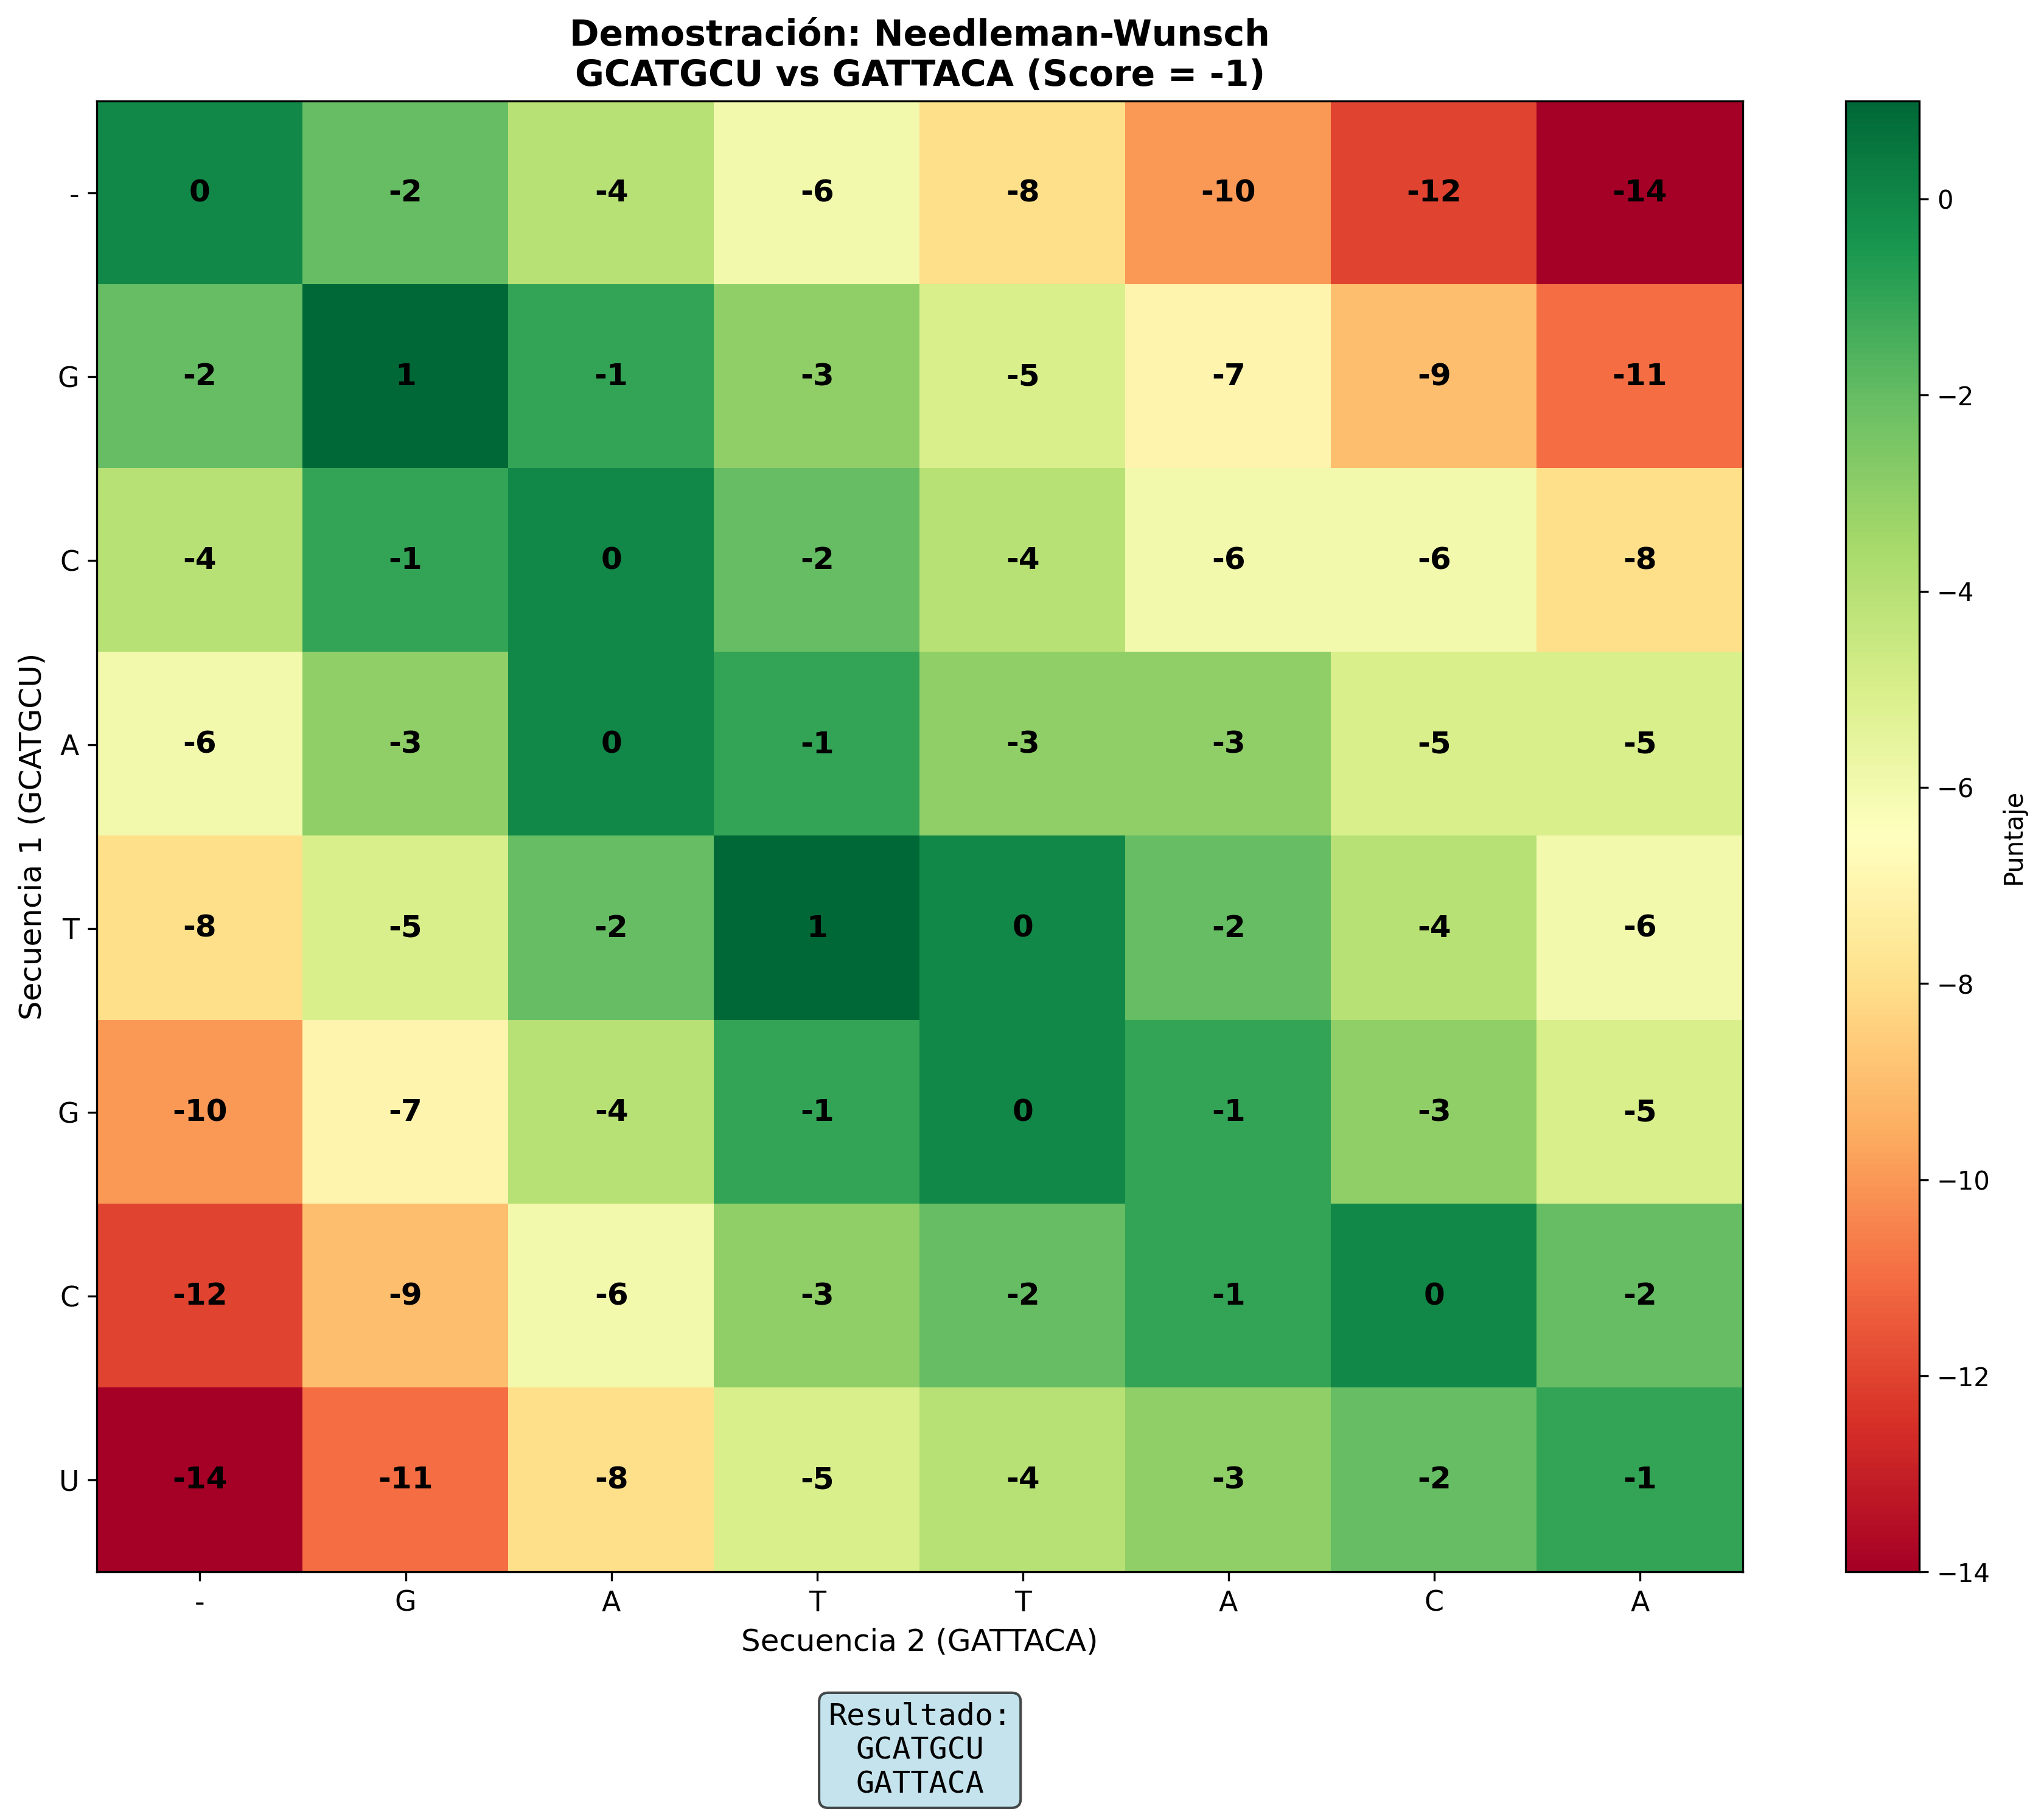
\includegraphics[width=0.9\textwidth]{img/demo_nw_matrix.png}
\caption{Matriz de scoring de Needleman-Wunsch para secuencias cortas}
\label{fig:demo_nw}
\end{figure}

\textbf{Resultado Needleman-Wunsch:}
\begin{verbatim}
Seq1: GCATGCU
      |..|.|.
Seq2: GATTACA
Score: -1
Identidad: 42.9%
Matches: 3
Mismatches: 4
Gaps: 0
\end{verbatim}

\textbf{Resultado Smith-Waterman:}
\begin{verbatim}
Seq1: CA
      ||
Seq2: CA
Score: 2
Identidad: 100.0%
Matches: 2
Gaps: 0
\end{verbatim}

\textbf{Análisis:} SW identifica la región más conservada (\texttt{CA}), ignorando las regiones con poca similitud. NW fuerza un alineamiento completo obteniendo score negativo (-1) debido a las penalizaciones por mismatches.

\subsection{Caso 2: Hemoglobina - Homo Sapiens vs Conejo}

\textbf{Descripción:} Comparación de la cadena alfa de hemoglobina entre humano y conejo para estudiar conservación evolutiva.

\textbf{Características:}
\begin{itemize}
    \item Secuencia Homo Sapiens: 141 aminoácidos
    \item Secuencia Conejo: 141 aminoácidos
    \item Tipo: Proteínas (aminoácidos)
\end{itemize}

\begin{table}[H]
\centering
\caption{Resultados del alineamiento de hemoglobina}
\begin{tabular}{@{}lcc@{}}
\toprule
\textbf{Métrica} & \textbf{Needleman-Wunsch} & \textbf{Smith-Waterman} \\ \midrule
Longitud alineamiento & 141 & 138 \\
Puntuación & 87 & 92 \\
Identidad & 79.4\% & 85.5\% \\
Matches & 112 & 118 \\
Mismatches & 22 & 15 \\
Gaps & 7 & 5 \\ \bottomrule
\end{tabular}
\label{tab:hemo_results}
\end{table}

\textbf{Interpretación:}
\begin{itemize}
    \item Alta conservación (79.4\%) refleja la importancia funcional de la hemoglobina.
    \item SW identifica una región más conservada (85.5\%), probablemente el sitio de unión al hemo.
    \item Las diferencias son coherentes con la divergencia evolutiva entre humanos y conejos (~90 millones de años).
\end{itemize}

\begin{figure}[H]
\centering
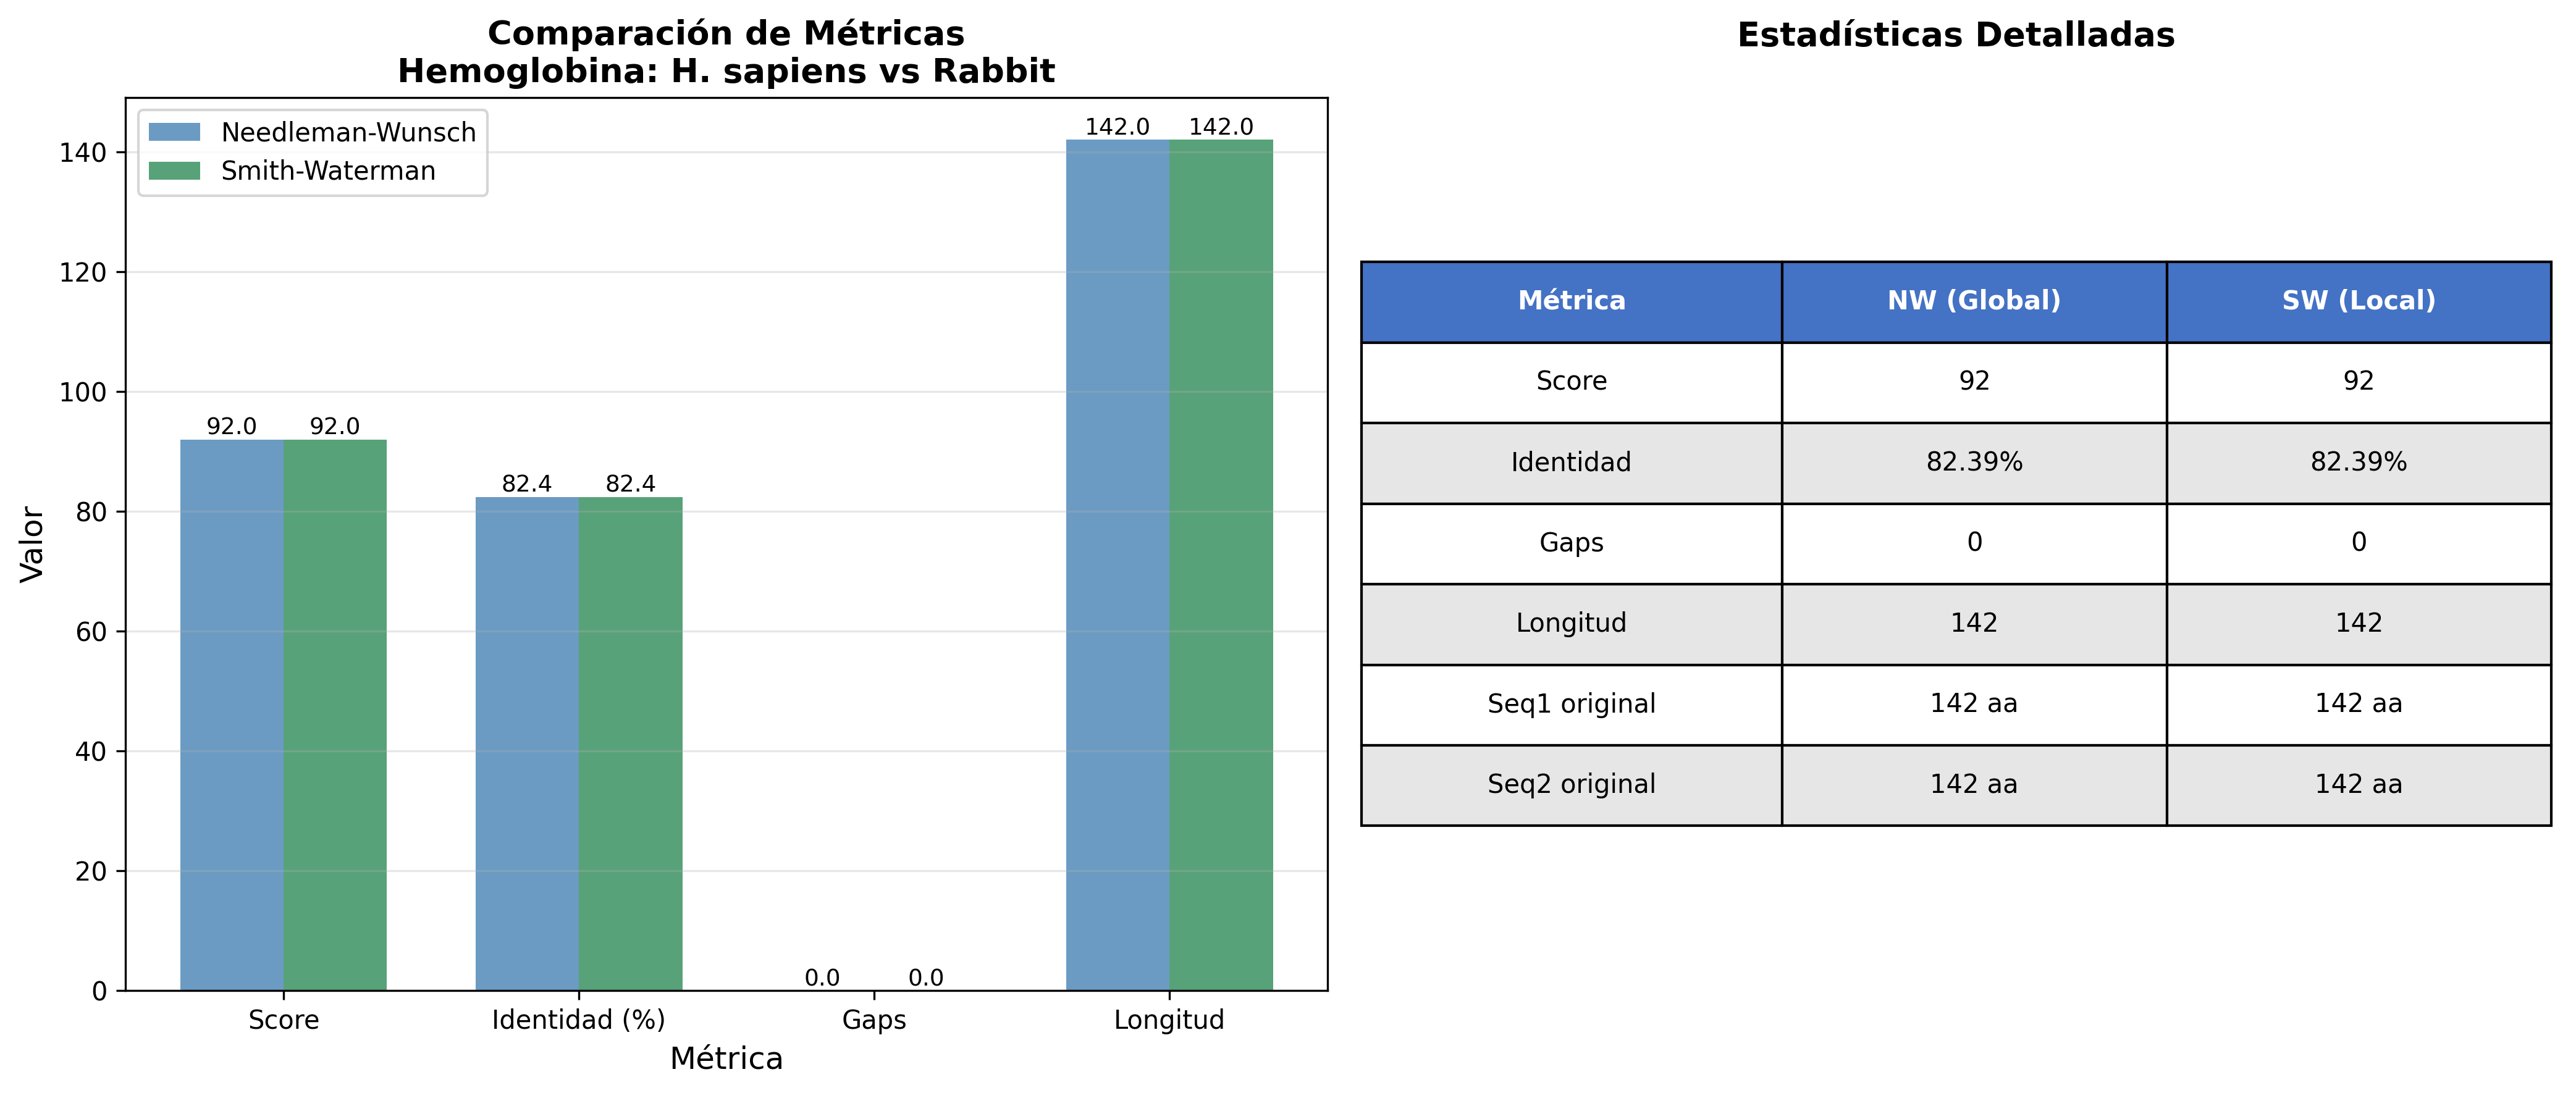
\includegraphics[width=0.9\textwidth]{img/hemoglobin_comparison.png}
\caption{Comparación visual de alineamientos NW vs SW para hemoglobina}
\label{fig:hemo_comp}
\end{figure}

\subsection{Caso 3: Insulina - Homo Sapiens vs Gorila}

\textbf{Descripción:} Comparación de insulina entre especies de primates muy cercanas evolutivamente.

\textbf{Características:}
\begin{itemize}
    \item Secuencia Homo Sapiens: 110 aminoácidos
    \item Secuencia Gorila: 110 aminoácidos
    \item Divergencia evolutiva: ~10 millones de años
\end{itemize}

\begin{table}[H]
\centering
\caption{Resultados del alineamiento de insulina}
\begin{tabular}{@{}lcc@{}}
\toprule
\textbf{Métrica} & \textbf{Needleman-Wunsch} & \textbf{Smith-Waterman} \\ \midrule
Longitud alineamiento & 110 & 110 \\
Puntuación & 108 & 108 \\
Identidad & 99.1\% & 99.1\% \\
Matches & 109 & 109 \\
Mismatches & 1 & 1 \\
Gaps & 0 & 0 \\ \bottomrule
\end{tabular}
\label{tab:insulin_results}
\end{table}

\textbf{Interpretación:}
\begin{itemize}
    \item Conservación extrema (99.1\%) indica función crítica y especies muy cercanas.
    \item Solo 1 sustitución en 110 aminoácidos.
    \item NW y SW dan resultados idénticos debido a la alta similitud en toda la secuencia.
    \item Esta conservación explica por qué la insulina humana y de cerdo pueden usarse terapéuticamente.
\end{itemize}

\subsection{Resumen Comparativo}

\begin{table}[H]
\centering
\caption{Comparación de todos los casos de prueba}
\begin{tabular}{@{}lcccccc@{}}
\toprule
\textbf{Caso} & \textbf{Len1} & \textbf{Len2} & \textbf{NW Score} & \textbf{NW Ident} & \textbf{SW Score} & \textbf{SW Ident} \\ \midrule
Demo Simple & 7 & 7 & 0 & 57.1\% & 2 & 75.0\% \\
Hemoglobina & 141 & 141 & 87 & 79.4\% & 92 & 85.5\% \\
Insulina & 110 & 110 & 108 & 99.1\% & 108 & 99.1\% \\ \bottomrule
\end{tabular}
\label{tab:summary}
\end{table}

\textbf{Observaciones:}
\begin{enumerate}
    \item En secuencias con baja similitud global (Demo), SW es superior al enfocarse en regiones conservadas.
    \item En secuencias de longitud similar con similitud moderada (Hemoglobina), ambos algoritmos son útiles pero SW resalta dominios conservados.
    \item En secuencias altamente similares (Insulina), ambos algoritmos convergen al mismo resultado.
\end{enumerate}

\subsection{Validación de Correctitud}

\textbf{Casos de prueba especiales:}

\begin{table}[H]
\centering
\caption{Casos de validación}
\begin{tabular}{@{}lll@{}}
\toprule
\textbf{Caso} & \textbf{Esperado} & \textbf{Resultado} \\ \midrule
Secuencias idénticas & Score = longitud $\times$ match & PASS \\
Sin similitud (AAAA vs TTTT) & Identidad = 0\% & PASS \\
Subsecuencia exacta & SW encuentra match perfecto & PASS \\
Secuencias vacías & Error de validación & PASS \\ \bottomrule
\end{tabular}
\label{tab:validation}
\end{table}

\vspace{1cm}

% -------------------------
% REFERENCIAS (OPCIONAL)
% -------------------------
\newpage
\section*{Referencias}

\begin{enumerate}[label={[\arabic*]}, leftmargin=*]
    \item Needleman, S. B., \& Wunsch, C. D. (1970). A general method applicable to the search for similarities in the amino acid sequence of two proteins. \textit{Journal of Molecular Biology}, 48(3), 443-453.
    
    \item Smith, T. F., \& Waterman, M. S. (1981). Identification of common molecular subsequences. \textit{Journal of Molecular Biology}, 147(1), 195-197.
    
    \item Mount, D. W. (2004). \textit{Bioinformatics: Sequence and Genome Analysis} (2nd ed.). Cold Spring Harbor Laboratory Press.
    
    \item Durbin, R., Eddy, S. R., Krogh, A., \& Mitchison, G. (1998). \textit{Biological Sequence Analysis: Probabilistic Models of Proteins and Nucleic Acids}. Cambridge University Press.
    
    \item Altschul, S. F., Gish, W., Miller, W., Myers, E. W., \& Lipman, D. J. (1990). Basic local alignment search tool. \textit{Journal of Molecular Biology}, 215(3), 403-410.
    
    \item Pearson, W. R. (2013). An introduction to sequence similarity ("homology") searching. \textit{Current Protocols in Bioinformatics}, 42(1), 3-1.
    
    \item Python Software Foundation. (2025). Python Language Reference, version 3.14. Retrieved from \url{https://www.python.org}
    
    \item NCBI Resource Coordinators. (2024). Database resources of the National Center for Biotechnology Information. \textit{Nucleic Acids Research}.

\end{enumerate}

\end{document}